% !TeX root = thesis.tex
%--------------------------------------------------------------------%
%
% Template TA LaTeX Teknik Informatika ITERA.
% Editor: Radhinka Bagaskara, Martin C.T. Manullang, iwawiwi
% Version 2024.1
%
% Berdasarkan "Templat LaTeX Tesis Informatika ITB" oleh Petra Barus & Peb Ruswono Aryan
% https://github.com/petrabarus/if-itb-latex
%--------------------------------------------------------------------%
%
% Berkas ini berisi struktur utama dokumen LaTeX yang akan dibuat.
%
%--------------------------------------------------------------------%

% Set jenis dokumen Tugas Akhir
\documentclass[12pt, a4paper, onecolumn, oneside, final]{report}

%-------------------------------------------------------------------%
%
% Konfigurasi dokumen LaTeX untuk laporan tesis IF ITB
% 
%
% @author Radhinka Bagaskara, Petra Novandi (ITB)
%
%-------------------------------------------------------------------%
%
% Berkas asli berasal dari Steven Lolong
%
%-------------------------------------------------------------------%

% Import package penting
\usepackage[utf8]{inputenc}
\usepackage{graphicx}
\usepackage{titling}
\usepackage{blindtext} % Untuk lorem ipsum
\usepackage{sectsty} % Untuk header & judul
\usepackage{chngcntr} % Untuk penambahan nomor caption
\usepackage{etoolbox} % Untuk CRUD variabel (?)
\usepackage{array} % % Untuk tabel di math mode
\usepackage{float} % Untuk tabular
\usepackage{longtable} % Untuk tabel yang potong halaman
\usepackage{amsmath} % Untuk equation
\usepackage{enumitem} % Untuk list enumerate yg lebih rapi
\usepackage[bookmarks]{hyperref}
\hypersetup{
	colorlinks,
	citecolor=black,
	filecolor=black,
	linkcolor=black,
	urlcolor=black
}

% Ukuran kertas A4
\special{papersize=210mm,297mm}

% Setting margin
\usepackage[top=3cm,bottom=3cm,left=3.5cm,right=3cm]{geometry}

% Setting indensasi
\usepackage{indentfirst}
\usepackage{parskip}
\setlength{\parindent}{20pt}
\setlength{\parskip}{10pt}

% Linespacing 1.5. Tidak serupa dengan 1.5 di Word (RDB)
\renewcommand{\baselinestretch}{1.5}

% Agar tidak ada kata yang terpotong setiap baris kalimat
\hyphenpenalty=10000

% Font
%\usepackage{mathptmx} 
\usepackage{newtx} 
% Times New Roman itu copyright dari Microsoft. Ini alternatifnya (RDB)

% Judul bahasa Indonesia
\usepackage[bahasa]{babel}

% Format tanggal
\usepackage[style=ddmmyyyy,datesep=-]{datetime2}

% Format citation
\usepackage[backend=bibtex,citestyle=ieee]{biblatex}

% Package untuk link di daftar isi.
\usepackage{titlesec}       % Package Format judul
\usepackage{parskip}
\usepackage{ragged2e}		% Alignment
\usepackage{multirow}		% Untuk bisa merge cell di tabel
\usepackage{tikz}			% Untuk menggambar kotak pas foto
\usepackage{setspace}		% Spacing paragraph
\usepackage{fancyhdr}		% Agar nomor halaman di pojok kanan atas
\usepackage{caption} 		% Caption gambar & tabel

% Setting supaya nomor halaman pertama dengan "chapter"
% berada di kanan atas
\fancypagestyle{plain}{%
	\fancyhf{}%
	\renewcommand{\headrulewidth}{0pt}
	\fancyhead[R]{\thepage}
}

% Setting judul
\chapterfont{\centering \large}
\titleformat{\chapter}[display]%
  	{\large\centering\bfseries}%
  	{\chaptertitlename\ \thechapter}{0pt}%
  	{\large\bfseries\uppercase}
\titleformat{\section}%
	{\normalfont\normalsize\bfseries}{\thesection}{1em}{}
\titleformat{\subsection}%
	{\normalfont\normalsize\bfseries}{\thesubsection}{1em}{}
    
% Setting spacing di setiap judul chapter
\titlespacing*{\chapter}{0pt}{-30pt}{20pt}

% Setting nomor pada subbsubsubbab
\setcounter{secnumdepth}{3}

% Counter untuk figure dan table, agar bertambah walaupun lintas subbab
\counterwithout{figure}{section}
\counterwithout{table}{section}

% Supaya tidak ada garis di header
\renewcommand{\headrulewidth}{0pt}

% Setting penomoran caption gambar
\renewcommand{\thefigure}{\arabic{chapter}.\arabic{figure}}

% Setting penomoran caption tabel
\renewcommand{\thetable}{\arabic{chapter}.\arabic{table}}

% Setting penomoran caption persamaan
\usepackage{tocloft}
% ---------------------------
% Custom List of Equations
% ---------------------------
\newcommand{\listequationsname}{\LARGE Daftar Persamaan}
\newlistof{myequations}{loe}{\listequationsname}

\renewcommand{\cftloetitlefont}{\hfill\Huge\bfseries}
\renewcommand{\cftafterloetitle}{\hfill}
\setlength{\cftafterloetitleskip}{10pt}
	
\newcommand{\myequations}[1]{%
  \addcontentsline{loe}{myequations}{\protect\numberline{\theequation}#1}%
}

\setlength{\cftmyequationsnumwidth}{2.3em}
\setlength{\cftmyequationsindent}{1.5em}
\renewcommand\theequation{\arabic{section}.\arabic{equation}}
% Mengkapitalkan judul Daftar Isi, Gambar, & Tabel
\addto\captionsbahasa{%
	\renewcommand{\contentsname}{DAFTAR ISI}%
	\renewcommand{\listfigurename}{DAFTAR GAMBAR}%
	\renewcommand{\listtablename}{DAFTAR TABEL}%
}

% Untuk mengganti nama bulan di babel bahasa
% tapi belum jalan (RDB)
\StartBabelCommands*{bahasa}{date}
\SetStringLoop{month#1name}{%
	Januari,Februari,Maret,April,Mei,Juni,%
	Juli,Agustus,September,Oktober,November,%
	Desember}
\EndBabelCommands     

% english title
\providecommand\titleEN[1]{\providecommand\thetitleEN{#1}}

% Saya lupa ini buat apa (RDB)
%\renewcommand{\theHsection}{\thepart.section.\thesection}

% Semua dibawah ini berhubungan dengan CRUD variabel (ada simbol @)
\makeatletter % Jangan dihapus

% Command untuk variabel NIM
\newcommand{\nim}[1]{\def\@nim{#1}}
\newcommand{\printnim}{\@nim}

% Command untuk variabel Dosen Pembimbing I & II
\newcommand{\namadosbinga}[1]{\def\@namadosbinga{#1}}
\newcommand{\namadosbingb}[1]{\def\@namadosbingb{#1}}
\newcommand{\nipdosbinga}[1]{\def\@nipdosbinga{#1}}
\newcommand{\nipdosbingb}[1]{\def\@nipdosbingb{#1}}
\newcommand{\printnamadosbinga}{\@namadosbinga}
\newcommand{\printnamadosbingb}{\@namadosbingb}
\newcommand{\printnipdosbinga}{\@nipdosbinga}
\newcommand{\printnipdosbingb}{\@nipdosbingb}
\newcommand{\dosbingA}[2]{\namadosbinga{#1} \nipdosbinga{#2}}
\newcommand{\dosbingB}[2]{\namadosbingb{#1} \nipdosbingb{#2}}

% Command untuk variabel Dosen Penguji I & II
\newcommand{\namapengujia}[1]{\def\@namapengujia{#1}}
\newcommand{\namapengujib}[1]{\def\@namapengujib{#1}}
\newcommand{\nippengujia}[1]{\def\@nippengujia{#1}}
\newcommand{\nippengujib}[1]{\def\@nippengujib{#1}}
\newcommand{\printnamapengujia}{\@namapengujia}
\newcommand{\printnamapengujib}{\@namapengujib}
\newcommand{\printnippengujia}{\@nippengujia}
\newcommand{\printnippengujib}{\@nippengujib}
\newcommand{\pengujiA}[2]{\namapengujia{#1} \nippengujia{#2}}
\newcommand{\pengujiB}[2]{\namapengujib{#1} \nippengujib{#2}}

% Command untuk merubah spacing equation
\g@addto@macro\normalsize{%
	\setlength\abovedisplayskip{-10pt}
	\setlength\belowdisplayskip{-10pt}
	\setlength\abovedisplayshortskip{-10pt}
	\setlength\belowdisplayshortskip{-10pt}
}

\makeatother % Jangan dihapus



\bibliography{references}

\begin{document}
% 	\pagestyle{plain}
% 	\fancyhf{}
% 	\rfoot{Halaman \thepage}%

    %----------------------------------------------------------------%
    % Konfigurasi Informasi Tugas Akhir
    %----------------------------------------------------------------%
    
    % Judul Tugas Akhir
    \title{ANALISIS METODE OVERSAMPLING SMOTE DAN ADASYN PADA RANDOM FOREST DAN XGBOOST DALAM MENANGANI SISTEM PENDETEKSI PENIPUAN KARTU KREDIT} 	
    % DITULIS DALAM HURUF KAPITAL; Font size 16 pt; Bold; Tidak melebihi 4 baris
    \titleEN{Analysis of SMOTE and ADASYN Oversampling Methods in Random Forest and Advanced Gradient Boosting Techniques in Handling Credit Card Fraud Detection Systems}      % Judul Tugas Akhir dalam Bahasa Inggris
    
    % Informasi Mahasiswa
    \author{Raihan Alghiffari}		% Nama Mahasiswa
	\nim{120140005}			% NIM Mahasiswa
	
	%Informasi Dosen Pembimbing
	\dosbingA%
		{Nama dan Gelar Pembimbing I}%	% Nama Dosen Pembimbing 1
		{NIP. 123456789}				% NIP Dosen Pembimbing 1
	\dosbingB%
		{Nama dan Gelar Pembimbing II}%	% Nama Dosen Pembimbing 2
		{NIP. 123456789}				% NIP Dosen Pembimbing 2
		
	%Informasi Dosen Penguji
	\pengujiA%
		{Nama dan Gelar Penguji I}%	% Nama Dosen Penguji 1
		{NIP. 123456789}				% NIP Dosen Penguji 1
	\pengujiB%
		{Nama dan Gelar Penguji II}%	% Nama Dosen Penguji 2
		{NIP. 123456789}				% NIP Dosen Penguji 2

	\sloppy % mencegah text overflow. (Jose)
    \pagenumbering{roman}
    \setcounter{page}{1} % Nomor halaman dimulai dengan "ii" di hal. Pengesahan

    \clearpage
\pagestyle{empty}

\begin{center}
	\smallskip
	
	\begin{center}
		\fontsize{16pt}{14pt}
		\bfseries \MakeUppercase{\thetitle}
		\vfill
	    \uppercase{Tugas Akhir}
	    \vfill
		\normalfont Diajukan sebagai syarat menyelesaikan jenjang strata Satu (S-1) di Program Studi Teknik Informatika, Jurusan Teknologi, Produksi dan Industri, Institut Teknologi Sumatera
		\vfill
	\end{center}

	\large \bfseries Oleh:\\
    \large \bfseries \theauthor\\
    \printnim
    \vfill
    
    \begin{figure}[h]
    	\centering
    	
\includegraphics[width=5cm, keepaspectratio]{resources/itera-logo}
    \end{figure}
    \vfill

	\begin{center}
		\fontsize{14pt}{16pt}
	    \bfseries
	    \uppercase{
	        Program Studi Teknik Informatika \\
	        Fakultas Teknologi Industri\\
	        Institut Teknologi Sumatera\\
	        Lampung Selatan
	    }\\
	    \the\year{}
    \end{center}

\end{center}

\clearpage
 % Hardcover
    \clearpage
\pagestyle{fancy}
\fancyhf{}
\fancyhead[R]{\thepage}
\phantomsection% 
\addcontentsline{toc}{chapter}{Lembar Pengesahan}

\begin{center}

	\large \bfseries \MakeUppercase{Lembar Pengesahan}
    
    \normalsize \normalfont \onehalfspacing \justify{
    Tugas Akhir Sarjana dengan judul "{\thetitle}" adalah benar dibuat oleh saya sendiri dan belum pernah dibuat dan diserahkan sebelumnya, baik sebagian ataupun seluruhnya, baik oleh saya ataupun orang lain, baik di Institut Teknologi Sumatera maupun di institusi pendidikan lainnya.}

	% Informasi Mahasiswa
	\setlength{\tabcolsep}{0pt}
	\begin{tabular}{p{0.7\textwidth} p{0.3\textwidth}}
		Lampung Selatan, \today & %
		\multirow{6}{*}{
			% Kotak pasfoto 3x4
			\phantom{---} % Amazing hack biar kotaknya ke kanan (RDB)
			\begin{tikzpicture}
				\draw rectangle (3cm,4cm) node[pos=0.5] {Foto 3x4};
			\end{tikzpicture}
		}\\
		Penulis, \\
		& \\
		& \\
		& \\
		& \\
		\theauthor\\
		NIM \printnim
	\end{tabular}

	% Informasi Dosen
	\centering Diperiksa dan disetujui oleh,
	\justify
    \setlength{\tabcolsep}{0pt}
    \begin{tabular}{ m{0.5cm}  m{0.7\textwidth} >{\centering\arraybackslash}m{0.3\textwidth}}
        \multicolumn{2}{c}{Pembimbing} & \multicolumn{1}{c}{Tanda Tangan} \\
		1. & \printnamadosbinga & \\
		 & \printnipdosbinga & ......................\\
		2. & \printnamadosbingb & \\
		 & \printnipdosbingb & ......................\\
		 & \\
		\multicolumn{2}{c}{Penguji} & \multicolumn{1}{c}{Tanda Tangan} \\
		1. & \printnamapengujia & \\
		& \printnippengujia & ......................\\
		2. & \printnamapengujib & \\
		& \printnippengujib & ......................\\
    \end{tabular}
%	\vfill

	\begin{center}
		\fontsize{10pt}{12pt}
		Disahkan oleh,\\
		Koordinator Program Studi Teknik Informatika\\
		Fakultas Teknologi Industri\\
		Institut Teknologi Sumatera
		\vspace{1.5cm}\\
		Andika Setiawan, S.Kom., M.Cs. \\ % TODO: make automatic
		NIP 19911127 2022 03 1 007 \\
	\end{center}
	\vfill

\end{center}
\clearpage
 % Lembar Pengesahan
    \clearpage
\phantomsection% 
\addcontentsline{toc}{chapter}{Halaman Pernyataan Orisinalitas}

\begin{center}
	\smallskip
	
%	\chapter*{\normalsize{Halaman Pernyataan Orisinalitas}}
	\large \bfseries \MakeUppercase{Halaman Pernyataan Orisinalitas} \linebreak
	
	\normalsize \onehalfspacing{
		Tugas Akhir dengan judul “{\thetitle}” adalah karya saya sendiri, dan semua sumber baik yang dikutip maupun dirujuk telah saya nyatakan benar. }
	\vspace{3cm}
	
	\centering 
	\begin{tabular}{l l}
		Nama 			& : \theauthor \\
		& \\
		NIM 			& : \printnim \\
		& \\
		\\
		Tanda Tangan 	& : ................................... \\
		& \\
		Tanggal 		& : ................................... \\
	\end{tabular}
	
\end{center}
\clearpage
 % Halaman Pernyataan Orisinalitas
    \clearpage
\phantomsection% 
\addcontentsline{toc}{chapter}{Halaman Persetujuan Publikasi}

\begin{center}
	\smallskip
	
	\normalsize \bfseries \MakeUppercase{
		HALAMAN PERNYATAAN PERSETUJUAN PUBLIKASI \\
		TUGAS AKHIR UNTUK KEPENTINGAN AKADEMIS
	}\linebreak
	
	\normalsize \normalfont \onehalfspacing \justifying
	Sebagai civitas akademik Institut Teknologi Sumatera, saya yang bertanda tangan di bawah ini:
	
	\flushleft
	\setlength{\tabcolsep}{0pt}
	\begin{tabular}{l l}
		Nama 			&  : \theauthor\\
		NIM 			&  : \printnim\\
		Program Studi \	&  : Teknik Informatika\\
		Fakultas 		&  : Teknologi Industri\\
		Jenis Karya 	&  : Tugas Akhir\\
	\end{tabular}

	\justifying
	\noindent demi pengembangan ilmu pengetahuan, menyetujui untuk memberikan kepada Institut Teknologi Sumatera \textbf{Hak Bebas Royalti Noneksklusif \textit{(Non-exclusive Royalty Free Right)}} atas karya ilmiah saya yang berjudul:
	
	\centering
	\textbf{\thetitle}
	
	\justifying
	beserta perangkat yang ada (jika diperlukan). Dengan Hak Bebas Royalti Noneksklusif ini Institut Teknologi Sumatera berhak menyimpan, mengalihmedia/formatkan, mengelola dalam bentuk pangkalan data (\textit{database}), merawat, dan memublikasikan tugas akhir saya selama tetap mencantumkan nama saya sebagai penulis/pencipta dan sebagai pemilik Hak Cipta.
	
	Demikian pernyataan ini saya buat dengan sebenarnya. \\
	
	\centering
	Dibuat di : Lampung Selatan\\
	Pada tanggal : \today\\ % Format bulan harusnya nama panjang, belum kepikiran gimana caranya (RDB)
	\bigskip
	Yang menyatakan\\
	\vspace{2cm}
	\theauthor
	
\end{center}
\clearpage
 % Halaman Persetujuan Publikasi
    \clearpage
\phantomsection% 
\addcontentsline{toc}{chapter}{Kata Pengantar}
\thispagestyle{fancy}

\begin{justifying}
	\large \bfseries \centering \MakeUppercase{Kata Pengantar}
	
	\normalsize \normalfont \justifying
	\textit{Pada halaman ini mahasiswa berkesempatan untuk menyatakan terima kasih secara tertulis kepada pembimbing dan pihak lain yang telah memberi bimbingan, nasihat, saran dan kritik, kepada mereka yang telah membantu melakukan penelitian, kepada perorangan atau lembaga yang telah memberi bantuan keuangan, materi dan/atau sarana. Cara menulis kata pengantar beraneka ragam, tetapi hendaknya menggunakan kalimat yang baku. Ucapan terima kasih agar dibuat tidak berlebihan dan dibatasi pada pihak yang terkait secara ilmiah (berhubungan dengan subjek/materi penelitian). } \par
	
	\textbf{Contoh}:\par
	Puji syukur kehadirat Allah SWT atas limpahan rahmat, karunia, serta petunjuk-Nya sehingga penyusunan tugas akhir ini telah terselesaikan dengan baik. Dalam penyusunan tugas akhir ini penulis telah banyak mendapatkan arahan, bantuan, serta dukungan dari berbagai pihak. Oleh karena itu pada kesempatan ini penulis mengucapan terima kasih kepada: \par
	\begin{enumerate}
		\item {[isi dengan nama Rektor ITERA]}
		\item {[isi dengan nama Dekan FTI]}
		\item {[isi dengan nama Kaprodi IF]}
		\item {[isi dengan nama Koordinator TA]}
		\item {[isi dengan nama Dosen Pembimbing]}
		\item {[isi dengan nama Orang Tua, Keluarga, dan kerabat lainnya]}
		\item {[isi dengan nama lain-lain]}
	\end{enumerate} \par
	Akhir kata penulis berharap semoga tugas akhir ini dapat memberikan manfaat bagi kita semua, amin. 
	\vfill
	
\end{justifying}
\clearpage
 % Kata Pengantar
    
    \clearpage
\phantomsection% 
\addcontentsline{toc}{chapter}{Ringkasan}
\thispagestyle{fancy}

\begin{center}
	\large \bfseries \MakeUppercase{Ringkasan}\\
	\normalsize \normalfont {\thetitle}\\
	\normalsize \normalfont {\theauthor}\\
	\bigskip
	
	\normalsize \normalfont \justifying
	Halaman Ringkasan berisi uraian singkat tentang latar belakang masalah, rumusan masalah, tujuan, metodologi penelitian, hasil dan analisis data, serta kesimpulan dan saran. Isi ringkasan tidak lebih dari 1500 kata (sekitar 3 halaman).\par
	
	\vfill
	
\end{center}
\clearpage % Ringkasan
    \clearpage
\phantomsection% 
\addcontentsline{toc}{chapter}{Abstrak}
\thispagestyle{fancy}

\begin{center}
	\large \bfseries \MakeUppercase{Abstrak}\\
	\normalsize \normalfont {\thetitle}\\
	\normalsize \normalfont {\theauthor}\\
	\bigskip
	
	\normalsize \normalfont \justifying \singlespacing
	Halaman ABSTRAK berisi uraian tentang latar belakang, tujuan, metodologi penelitian, hasil / kesimpulan. Ditulis dalam BAHASA INDONESIA tidak lebih dari 250 kata, dengan jarak antar baris satu spasi. \par
	
	Pada akhir abstrak ditulis kata “Kata Kunci” yang dicetak tebal, diikuti tanda titik dua dan kata kunci yang tidak lebih dari 5 kata. Kata kunci terdiri dari kata-kata yang khusus menunjukkan dan berkaitan dengan bahan yang diteliti, metode/instrumen yang digunakan, topik penelitian. Kata kunci diketik pada jarak dua spasi dari baris akhir isi abstrak.\par
	
	\textbf{Kata Kunci: Kata Kunci 1, Kata Kunci 2}
	
	\vfill
	
\end{center}
\clearpage % Abstrak (Indonesia)
    \clearpage
\phantomsection% 
\addcontentsline{toc}{chapter}{Abstract}
\thispagestyle{fancy}

\begin{center}
	\large \bfseries \MakeUppercase{Abstract}\\
	\normalsize \normalfont {\thetitleEN}\\
	\normalsize \normalfont {\theauthor}\\
	\bigskip
	
	\normalsize \normalfont \justifying \singlespacing
	Halaman ABSTRACT berisi uraian tentang latar belakang, tujuan, metodologi penelitian, hasil / kesimpulan. Ditulis dalam BAHASA INGGRIS tidak lebih dari 250 kata, dengan jarak antar baris satu spasi. Secara khusus, kata dan kalimat pada halaman ini tidak perlu ditulis dengan huruf miring meskipun menggunakan Bahasa Inggris, kecuali terdapat huruf asing lain yang ditulis dengan huruf miring (misalnya huruf Latin atau Greek, dll). \par
	
	Pada akhir abstract ditulis kata “Keywords” yang dicetak tebal, diikuti tanda titik dua dan kata kunci yang tidak lebih dari 5 kata. Keywords terdiri dari kata-kata yang khusus menunjukkan dan berkaitan dengan bahan yang diteliti, metode/instrumen yang digunakan, topik penelitian. Keywords diketik pada jarak dua spasi dari baris akhir isi abstrak.\par
	
	\textbf{Keywords: Kata Kunci 1, Kata Kunci 2}
	
	\vfill
	
\end{center}
\clearpage % Abstrak (Inggris)
%    \clearpage

\normalsize \bfseries \centering \MakeUppercase{Motto}
\phantomsection% 
\addcontentsline{toc}{chapter}{Motto}
\\[2\baselineskip]

\justifying \normalfont{
	% Motto
	\blindtext
}

\clearpage
%    \clearpage

% PS: Ada bug dimana jika menge-build dari file ini, ada error. Tapi halamannya
% sendiri tidak error jika dibuild dari file lain. (Radhinka)

\normalsize \bfseries \centering \MakeUppercase{Persembahan}
\phantomsection% 
\addcontentsline{toc}{chapter}{Persembahan}
\\[2\baselineskip]

\justifying \normalfont{
	% Kata-kata persembahan
	\blindtext
}

\clearpage

    % Configuration every chapter of Tableof content/table/image
% ---------------------------
% Standard Lists (TOC, Tables, and Figures)
% ---------------------------
\renewcommand{\contentsname}{\LARGE Daftar Isi}
\renewcommand{\listtablename}{\LARGE Daftar Tabel}
\renewcommand{\listfigurename}{\LARGE Daftar Gambar}

\renewcommand{\cfttoctitlefont}{\hfill\Huge\bfseries}
\renewcommand{\cftaftertoctitle}{\hfill}
\setlength{\cftaftertoctitleskip}{10pt}

\renewcommand{\cftlottitlefont}{\hfill\Huge\bfseries}
\renewcommand{\cftafterlottitle}{\hfill}
\setlength{\cftafterlottitleskip}{10pt}

\renewcommand{\cftloftitlefont}{\hfill\Huge\bfseries}
\renewcommand{\cftafterloftitle}{\hfill}
\setlength{\cftafterloftitleskip}{10pt}

	\addcontentsline{toc}{chapter}{Daftar Isi}
	\tableofcontents
	\pagebreak
	% Daftar tabel

	\phantomsection% 
	\addcontentsline{toc}{chapter}{Daftar Tabel}
	\listoftables
	\pagebreak
	% Daftar gambar
	\phantomsection% 
	\addcontentsline{toc}{chapter}{Daftar Gambar}
	\listoffigures
	\pagebreak
	% Daftar persamaan
	\phantomsection% 
	\addcontentsline{toc}{chapter}{Daftar Persamaan}
	\listofmyequations
	\pagebreak
%    \clearpage

\chapter*{Daftar Simbol}
\thispagestyle{fancy}
\fancyhf{}
\fancyhead[R]{\thepage}

\justifying
(Tuliskan maksud penulisan laporan, misal “Laporan penelitian ini dimaksud kan untuk memenuhi salah ”.........Pada halaman ini mahasiswa berkesempatan untuk menyatakan terima kasih secara tertulis kepada pembimbing dan pihak lain yang telah memberi bimbingan, nasihat, saran dan kritik, kepada mereka yang telah membantu melakukan penelitian, kepada perorangan atau lembaga yang telah memberi bantuan keuangan, materi dan/atau sarana.

Cara menulis kata pengantar beraneka ragam, tetapi hendaknya menggunakan kalimat yang baku. Ucapan terima kasih agar dibuat tidak berlebihan dan dibatasi pada pihak yang terkait secara ilmiah (berhubungan dengan subjek/materi penelitian). 


    %----------------------------------------------------------------%
    % Konfigurasi Bab
    %----------------------------------------------------------------%
    \renewcommand{\chaptername}{BAB}
    % Bab: Arabic
    \renewcommand{\thechapter}{\Roman{chapter}}
    % Sub-bab: Roman
    \renewcommand\thesection{\arabic{chapter}.\arabic{section}}
    
    % Setting supaya nomor halaman pertama dengan "chapter"
    % berada di tengah bawah, tapi selanjut2nya di kanan atas
    \fancypagestyle{plain}{%
    	\fancyhf{}%
    	\renewcommand{\headrulewidth}{0pt}
    	\fancyhead[]{}
    	\fancyfoot[C]{\thepage}
    }
    % Reset penomoran halaman menjadi 1
    \setcounter{page}{1}
    \pagenumbering{arabic}
    
    %----------------------------------------------------------------%

    %----------------------------------------------------------------%
    % Daftar Bab
    % Untuk menambahkan daftar bab, buat berkas bab misalnya `chapter-6` di direktori `chapters`, dan masukkan ke sini.
    %----------------------------------------------------------------%
    \justifying
    \newpage
\newcommand{\kreditgede}{Your Value}

\chapter{Pendahuluan} \label{Bab I}
% TODO  DONE Revisi Later Belakang
\section{Latar Belakang} \label{I.Latar Belakang}
Kartu kredit merupakan alat pembayaran yang menggantikan uang tunai dalam transaksi. Dengan kartu kredit, tidak perlu membawa uang tunai, sehingga memberikan kemudahan dan mendorongpeningkatan penggunaannya\cite{setiawan2022perlindungan}. Namun, di balik segala kemudahan dan keuntungan yang manjadikan ketergantungan dalam penggunaan kartu kredit, terdapat satu masalah dalam penggunaan kartu kredit yaitu penipuan dalam transaksi kartu kredit\cite{hendarsyah2020analisis}. Berdasarkan data dari Experian, 60\% pengguna kartu kredit pernah mengalami penipuan kartu kredit yang mana memberikan kerugian yang besar bagi pengguna kartu kredit dan juga agensi kartu kredit\cite{experian_2024} dan bahkan menurut analisis \textit{Merchant Cost Consulting} kerugian dari transaksi penipuan kartu kredit akan terus bertambah dan bisa mencapai 43 miliar dolar pada tahun 2026\cite{merchantcostconsulting_2024}.

Penipuan kartu kredit bisa berupa penipuan kartu kredit internal dan eksternal. Penipuan kartu kredit internal bisa terjadi karena persetujuan antara pemegang kartu dan bank dengan menggunakan identitas palsu untuk melakukan penipuan sedangkan penipuan kartu kredit eksternal melibatkan penggunaan kartu kredit curian untuk mendapatkan uang tunai\cite{chaudhary2012review}, dikarenakan itu mendeteksi penipuan kartu kredit menjadi masalah yang complex dan apabila mendeteksi penipuan kartu kredit secara manual memakan waktu yang banyak dan tidak efisien, disebabkan \textit{big data} yang sudah tidak memungkinankan metode manual bisa dilakukan. yang mana, lembaga keuangan sekarang lebih fokus kepada \textit{computational methodologies} sebagai metode yang lebih efisien dalam mengatasi penipuan kartu kredit\cite{west2016intelligent}.

Data mining merupakan salah satu \textit{computational methodologies} terbaik dalam mendeteksi penipuan kartu kredit, yang mana salah satu tekniknya yaitu klasifikasi yang dilakukan dengan cara membagi data menjadi dua kelas yaitu transaksi normal dan transaksi penipuan\cite{ngai2011application}. Sistem pendeteksi penipuan kartu kredit berkerja berdasarkan pada analisis perilaku pengguna kartu kredit dalam melakukan transaksi. Banyak teknik atau algoritma yang digunakan untuk mendeteksi penipuan kartu kredit seperti menggunakan neural network\cite{georgieva2019using}, genetic algorithm\cite{benchaji2019using}, frequent itemset mining\cite{seeja2014fraudminer}, support vector machine\cite{kumar2022credit}, decision tree\cite{gaikwad2014credit} dan lain-lain. 

Hasil dari teknik atau algoritma yang telah digunakan memberikan hasil yang berbeda-beda. untuk itu, ada beberapa metode dan tahap dalam memilih algoritma apa yang digunakan dalam mengembangkan model \textit{machine learning}, salah satu contohnya seperti melakukan komparasi beberapa algoritma machine learning untuk kasus yang sama dan menentukan yang hasil terbaik berdasarkan metode evaluasi yang ditentukan\cite{mniai2023novel}.

Masalah utama dalam membuat model pendeteksi penipuan kartu kredit ialah \textit{unbalance data} yang sangat berat antara transaksi penipuan dan transaksi normal yang membuat performa model menjadi sangat buruk dan perlu adanya preprocessing data terlebih dahulu seperti melakukan oversampling agar data yang diinputkan ke machine learning menjadi \textit{balance}sehingga menghasilkan performa yang baik\cite{mniai2023novel}.

Hasil riset-riset sebelumnya menunjukan bahwa algoritma \textit{esemble learning} merupakan algoritma terbaik dalam membuat model pendeteksi penipuan kartu kredit\cite{ningsih2022analisis}. \textit{Esemble learning} merupakan algoritma yang meningkatkan performa prediksi dan dapat mengatasi \textit{complex relationships} di sebuah machine learning dengan memanfaatkan \textit{multiple decision trees} salah satu contoh  algoritma esemble learning ialah random forest dan xgboost\cite{dietterich2002ensemble}.

Beberapa riset sebelumnya berfokus pada metode komparasi model machine learning guna menentukan model machine learning terbaik dalam membuat model pendeteksi penipuan kartu kredit\cite{mniai2023novel}. Namun, ada hal krusial yang jarang dijadikan fokus dalam penelitian yaitu process metode oversampling untuk mengatasi umbalance data, penggunaan metode oversampling yang berbeda-beda akan menghasilkan hasil performa yang berbeda-beda\cite{liu2004effect}. Metode oversampling yang digunakan dalam penelitian ini ialah \textit{synthetic minority over-sampling technique}(SMOTE)\cite{chawla2002smote} dan \textit{adaptive synthetic sampling}(ADASYN)\cite{4633969} dikarenakan metode tersebut memberikan hasil yang selalu berbeda dan tidak saling mengungguli satu sama lain dan menghasilkan hasil yang baik dikasus yang berbeda-beda sesuai dengan pola dataset dan tujuan pembuatan model\cite{brandt2021comparative}.

Fokus utama dari riset penulis ialah melakukan \textit{comparative analysis} metode oversampling \textit{synthetic minority over-sampling}(SMOTE) dan \textit{adaptive synthetic sampling}(ADASYN) dengan menggunakan algoritma esemble learning seperti random forest dan xgboost dalam membuat model pendeteksi penipuan kartu kredit dengan menggunakan metode evaluasi \textit{precision}, \textit{recall}, \textit{f1-score}, dan \textit{Matthews’s correlation coefficient} (MCC) \textit{metrics}. Dataset yang digunakan ialah dataset \textit{credit card fraud detection} yang dibuat dan dikumpulkan oleh grup machine learning dari \textit{Université Libre de Bruxelles}(ULB)\cite{dal2015calibrating}. Dataset ini berisi berisi 284807 transaksi kartu kredit yang dilakukan oleh pemegang kartu di  eropa  selama  dua  hari  dengan bobot  transaksi  normal  sebanyak  99,83\%  dan  fraud  sebanyak  0,17\% yang artinya dataset yang digunakan \textit{highly unbalanced}\cite{WinNT}. Riset kali ini akan memperluas penanganan \textit{unbalance data} penipuan kartu kredit untuk menentukan metode oversampling terbaik antara SMOTE dan ADASYN.
% TODO DONE Revisi Rumusan Masalah dan Tujuan
\section{Rumusan masalah} \label{I.Rumusan Masalah}
Berdasarkan latar belakang yang ada, rumusan masalah dalam penelitian ini sebagai berikut:

\begin{enumerate}[noitemsep]
        \item Bagaimana cara kerja algoritma oversampling SMOTE dan ADASYN dalam membuat data sintetis?
        \item Bagaimana kinerja metode oversampling SMOTE dan ADASYN dalam meningkatkan akurasi model Random Forest dan XGBoost dalam mendeteksi penipuan kartu kredit?
\end{enumerate}

\section{Tujuan} \label{I.Tujuan}
Adapun tujuan dari penelitian ini adalah sebagai berikut:
\begin{enumerate}[noitemsep]
        \item Mengetahui cara kerja algorimta oversampling SMOTE dan ADASYN dalam membuat data sintetis.
        \item Mengetahui kinerja model dengan oversampling SMOTE dan ADASYN dalam meningkatkan akurasi model Random Forest dan XGBoost dalam mendeteksi penipuan kartu kredit.
\end{enumerate}

\section{Batasan Masalah} \label{I.Batasan}
Batasan-batasan permasalahan dalam penelitian ini mencakup hal-hal berikut: 
\begin{enumerate}[noitemsep]
    \item Penelitian ini hanya menggunakan  dataset \textit{Credit Card Fraud Detection} dari kaggle dengan pengumpulannya berdasarkan hasil dari \textit{research collaboration} Université Libre de Bruxelles.
    \item Penelitian ini hanya akan menganalisis dua metode oversampling, yaitu SMOTE dan ADASYN, tanpa membandingkannya dengan metode oversampling atau undersampling lainnya.
    \item Analisis ini akan fokus pada dua algoritma machine learning, yaitu Random Forest dan Advanced Gradient Boosting Techniques seperti XGBoost tanpa mempertimbangkan algoritma lain seperti Support Vector Machine, Neural Networks, atau k-Nearest Neighbors.
\end{enumerate}

\section{Manfaat Penelitian} \label{I.Manfaat}
Adapun manfaat dari penelitian ini adalah sebagai berikut:
\begin{enumerate}[noitemsep]
    \item Mengetahui cara melakukan oversampling dengan metode SMOTE dan ADASYN
    \item Mengetahui cara membuat model Random Forest dan Advanced Gradient Boosting Techniques seperti XGBoost.
    \item Mengetahui metode oversampling terbaik diantara SMOTE dan ADASYN didalam sebuah algoritma Random Forest dan XGBoost untuk membuat model pendeteksi penipuan kartu kredit.
\end{enumerate}

% TODO DONE Revisi Sistematika Penulisan
\section{Sistematika Penulisan} \label{I.Sistematika}
Adapun sistematika penulisan dalam penelitian adalah sebagai berikut:
\subsection{Bab I Pendahuluan}
Bab ini merangkum beberapa hal yang berkaitan dengan penelitian yakni latar belakang, pengenalan masalah, perumusan pertanyaan penelitian, pendekatan metodologi, sasaran tujuan penelitian, batasan–batasan cakupan penelitian, dampak manfaat hasil penelitian, dan susunan sistematis penulisan.
\subsection{Bab II Tinjauan Pustaka}
Bab ini memfokuskan pada pengulasan tinjauan pustaka yang terkait dengan topik yang meliputi kartu kredit, SMOTE, ADASYN, Random Forest, XGBoost dan serta metode pengujian.
\subsection{Bab III Analisis Dan Perancangan}
Bab ini menguraikan tentang metodologi yang akan digunakan dalam penelitian. Ini meliputi pendekatan pembuatan model seperti pembuatan program, pengumpulan dataset, persiapan data, implementasi dan evaluasi terhadap program yang telah dirancang.
\subsection{Bab IV Hasil Dan Pembahasan}
Bab ini menjelaskan hasil dari penelitian yang telah dilakukan dan berisikan pembahasan dan analisis secara detail tentang kinerja metode oversampling SMOTE dan ADASYN dalam meningkatkan akurasi model pendeteksi penipuan kartu kredit.
\subsection{Bab V Kesimpulan Dan Saran}
Bab ini berisikan pembahasan tentang kesimpulan berdasarkan hasil dan pembahasan dari penelitian yang telah dilakukan dan juga terdapat saran yang dipaparrkan untuk pengembangan penelitian di masa yang akan datang. 

    \newpage
\chapter{Tinjauan Pustaka} \label{Bab II}

\section{Tinjauan Pustaka} \label{II.Tinjauan}
Pada penelitian ini, peneliti melakukan eksplorasi dan mendapatkan tinjauan pustaka berdasarkan penelitian sebelumnya yang berkaitan dengan pembangunan model pendeteksi penipuan kartu kredit. Peneliti menjadikan penelitian terdahulu sebagai referensi dan landasan perbandingan serta kajian terhadap penelitian yang akan dilakukan. Berikut penelitian-penelitian terdahulu yang berhubungan dengan penelitian ini:
\begin{enumerate}[noitemsep]
	\item Tahun 2021, Asha RB, Suresh Kumar KR,       melakukan penelitian terkait dengan \textit{Credit card fraud detection using artificial neural network}. Tujuan Penelitian ini ialah untuk membandingkan hasil dari traditional machine learning seperti SVM dan ANN. Hasil dari penelitian ini ialah menunjukan bahwa ANN lebih baik dibandingkan traditional machine learning berdasarkan accuracy \cite{asha2021credit}.
    \item Tahun 2021, Tayebi, Mohammed dan El Kafhali, melakukan penelitian terkait dengan \textit{Hyperparameter optimization using genetic algorithms to detect frauds transactions}. Tujuan penelitian ini bertujuan untuk menangani penipuan transaksi kartu kredit dengan menggunakan \textit{machine learning} untuk mendeteksi penipuan dengan menerapkan \textit{genetic algorithm}(GA) untuk mengoptimalkan hyperparameter dan melakukan komparasi dengan menggunakan \textit{grid search method}. Evaluasi yang digunakan ialah \textit{accuracy}, precision, \textit{recall}, dan \textit{F1 score}\cite{tayebi2021hyperparameter}.
    \item Tahun 2022, Putu Tirta Sari Ningsih, Muhammad Gusvarizon, Rudi Hermawan, melakukan penelitian terkait dengan Analisis sistem pendeteksi penipuan transaksi kartu kredit dengan algoritma machine learning. Tujuan penelitian ini ialah melakukan komparasi berbagai algoritma \textit{machine learning} seperti \textit{decision tree}, \textit{random forest}, \textit{logistic regression}, dan \textit{support vector machine} dalam membuat sistem pendeteksi penipuan transaksi kartu kredit. Evaluasi yang digunakan ialah \textit{accuracy}, \textit{precision}, \textit{recall}, \textit{F-1 score}, \textit{receiver operating characteristics}(ROC), \textit{area Under the Curve}(AUC), dan \textit{matthew coefficient score}(MCC). Hasil penelitian ini membuktikan ensemble learning algoritm seperti random forest merupakan algoritma terbaik dalam membuat sistem pendeteksi penipuan transaksi kartu kredit karena memiliki nilai performa keseluruhan paling baik dengan MCC 87\%\cite{ningsih2022analisis}.
    \item Tahun 2022, Kumar Sheo, Gunjan Vinit Kumar, Ansari Mohd Dilshad, Pathak, Rashmi, melakukan penelitian terkait dengan \textit{Credit card fraud detection using support vector machine}. Tujuan riset ini ialah menemukan sistem paling efektif dalam mengidentifikasi penipuan kartu kredit dengan menggunakan \textit{support vector machine} dalam  menglasifikasi penipuan dan normal transaksi kartu kredit dalam melakukan deteksi.\cite{kumar2022credit}.
    \item Tahun 2020, Ruttala Sailusha, V. Gnaneswar, R. Ramesh, dan G. Ramakot eswara Raom, melakukan penelitian terkait dengan \textit{Credit card fraud detection using machine learning}. Penelitian ini membandingkan dua algoritma \textit{ensemble learning} yaitu \textit{random forest} dan \textit{adaboost}. Evaluasi yang digunakan ialah \textit{accuracy}, \textit{precision}, \textit{recall}, \textit{F-1 score}. Hasil dari penelitian ini memberikan kesimpulan kalau walaupun banyaknya teknik deteksi penipuan dia tidak bisa bilang kalau algoritma bisa mendeteksi penipuan secara menyeluruh dan hasil komparasinya menunjukan kalau secara akurasi \textit{random forest} dan \textit{adaboost} menunjukan kesamaan namun secara \textit{precision}, \textit{recall}, \textit{F-1 score} \textit{random forest} lebih unggul. \cite{9121114}.
    \item Tahun 2024, Abdul Rehman Khalid, Nsikak Owoh, Omair Uthmani, Moses Ashawa, Jude Osamor, dan John Adejoh, melakukan penelitian terkait \textit{Enhancing credit card fraud detection: an ensemble machine learning approach}. Tujuan penelitian ini melakukan komparasi analisis terkait \textit{ensemble machine learning} seperti \textit{support vector machine} \textit{random forest} dan \textit{boosting classifiers}. Hasil dari penelitian ini mengaris bawahi bahwa ensemble methods merupakan tool yang terbaik untuk menangani kasus penipuan transaksi. \cite{khalid2024enhancing}
    \item Tahun 2023, Purwar, Archana and Manju, Ms, melakukan penelitian terkait \textit{Credit card fraud detection using XGBoost for imbalance dataset}. Tujuan dari penelitian ini ialah membuat model pendeteksi transaksi penipuan kartu kredit dengan menggunakan \textit{learning algorithm} xgboost. Hasil penelitian ini menunjukan bahwa xgboost menghasilkan performa model yang baik. \cite{purwar2023credit}
\end{enumerate}

\begin{longtable}{| >{\centering\arraybackslash}p{0.05\textwidth} |
                     >{\centering\arraybackslash}p{0.2\textwidth} |
                     >{\centering\arraybackslash}p{0.2\textwidth} |
                     >{\centering\arraybackslash}p{0.15\textwidth} |
                     >{\centering\arraybackslash}p{0.25\textwidth} |}
    \caption{Literasi Penelitian Terdahulu} % Caption only shown in the first table instance
    \label{table:2.literasi} \\
    \hline
    \textbf{No.} & \textbf{Judul} & \textbf{Masalah} & \textbf{Metode} & \textbf{Hasil} \\
    \hline
    \endfirsthead
    \hline
    \textbf{No.} & \textbf{Judul} & \textbf{Masalah} & \textbf{Metode} & \textbf{Hasil} \\
    \hline
    \endhead
    % Add your table content here
    1. & \textit{Credit card fraud detection using artificial neural network} & Penipuan dalam transaksi kartu kredit merupakan hal yang umum saat ini karena sebagian besar dari kita lebih sering menggunakan metode pembayaran kartu kredit. Hal ini disebabkan kemajuan teknologi dan peningkatan transaksi online mengakibatkan penipuan yang menyebabkan kerugian finansial yang sangat besar. & support vector machine (SVM), k-nearest neighbor (KNN), Artificial neural network (ANN) & SVM accuracy= 0.9349 precision= 0.9743 recall= 0.8976, KNN accuracy= 0.9982 precision= 0.7142 recall= 0.0393, dan ANN accuracy= 0.9992 precision= 0.8115 recall= 0.7619\\
    \hline
    2. & \textit{Hyperparameter optimization using genetic algorithms to detect frauds transactions} & sekarang servis online berkembang menjadi sangat besar dan maka dengan itu juga penipuan dalam servis online juga menjadi lebih besar, termasuk penipuan traksasi kartu kredit. & SMOTE, grid search (GS) methods, random forest (RF), AdaBoost (AB), logistic regression (LR), decision tree (DT), and support vector machine (SVM) classifier. & SVM: Precision=95\%, Recall=95\%, F1-score=95\%, Accuracy=94\%, Time=19.039
    LR: Precision=97\%, Recall=91\%, F1-score=94\%, Accuracy=94\%, Time=104.016
    AB: Precision=98\%, Recall=93\%, F1-score=95\%, Accuracy=95\%, Time=235.037
    RF: Precision=96\%, Recall=92\%, F1-score=94\%, Accuracy=94\%, Time=130.300
    DT: Precision=94\%, Recall=91\%, F1-score=93\%, Accuracy=92\%, Time=12.709\\
    \hline
    3. & Analisis sistem pendeteksi penipuan transaksi kartu kredit dengan algoritma machine learning & Banyaknya volume transaksi dan cepatnya proses transaksi yang berlangsung, membuat tidak mungkin untuk diawasi secara manual oleh manusia karena itu penpuan transaksi menjadi masalah dan harus diselesaikan dengan machine & analisis komparasi model + imbalance, model + SMOTE, model + param + imbalance, model + param + SMOTE, dengan model decision tree (DT), random forest (RF), logistic regression (LR), dan support vector machine (SVM) & algoritma random forest (RF) memiliki performa paling baik di antara semua model, disusul oleh model dengan algoritma decision tree (DT), hal ini pula yang membuktikan bahwa ensemble learning adalah teknik terbaik untuk fraud detection.\\
    \hline
    4. & \textit{Credit card fraud detection using support vector machine} & Penipuan kartu kredit tidak diragukan lagi merupakan ekspresi penipuan kriminal. Identifikasi penipuan tampaknya menjadi masalah rumit yang memerlukan banyak keterampilan hingga memasukkan algoritma terkait pembelajaran mesin ke dalamnya. & SVM & Hasil simulasi menunjukan bahwa SVM lebih baik dibandingkan \textit{state of art approaches}. \\
    \hline
    5. & \textit{Credit card fraud detection using machine learning} & Deteksi penipuan kartu kredit saat ini paling banyak dilakukan karena permasalahannya yang sering terjadi di dunia saat ini. hal ini disebabkan peningkatan transaksi online dan platform e-commerce & Adaboost dan Random Forest & Random Forest precision= 0.97\% recall= 89\% f1-score= 0.93 AUC=94\%, Adaboost precision= 89\% recall= 81,5\% f1-score= 84,5\% AUC=96\%.\\
    \hline
    6. & \textit{Enhancing credit card fraud detection: an ensemble machine learning approach} & Di era kemajuan digital, meningkatnya penipuan kartu kredit mengharuskan adanya pengembangan sistem deteksi penipuan yang kuat dan efisien. & /textit{Compare} ensemble learning dan traditional machine learning Support Vector Machine (SVM), K-Nearest Neighbor (KNN), Random Forest (RF), Bagging, and Boosting classifiers. & Metode ensamble mengungguli model individual, menunjukkan efektivitas penggabungan beberapa model. \\
    \hline
    7. & \textit{Credit card fraud detection using XGBoost for imbalanced data set} & Peningkatan tingkat penipuan di seluruh dunia, berbagai algoritma pembelajaran mesin digunakan oleh analis dan peneliti untuk mendeteksi dan menganalisis penipuan dalam transaksi online. Namun, kumpulan data pelatihan mungkin memiliki beberapa instance dari satu atau lebih instance dari kelas lain dalam kasus klasifikasi biner kelas tertentu yang membuat hasilnya menjadi bias. & XGBOOST & F1 score, recall and accuracy as 82.78\%, 78.9\% and 99.3\% \\
    \hline
\end{longtable}

\section{Dasar Teori} \label{II.Teori}
\subsection{Machine Learning} \label{II.Dasar Teori}
\textit{Machine learning} merupakan sebuah algoritma yang dapat membuat komputer belajar tanpa diprogram secara langsung\cite{alpaydin2021machine}. Kemampuan untuk belajar dan menentukan pilihan berdasarkan hasil pembelajaran, membuat \textit{Machine Learning} sering disebut sebagai AI atau \textit{Artificial Intelligence}. Namun, kenyataannya itu merupakan sub divisi dari AI dan pada tahun 1970an baru menjadi bagian dari evolusi AI dikarenakan sebelum tahun tersebut peneliti lebih berfokus kepada pendekatan \textit{logical} dan \textit{knowledge-based} dibandingkan algoritma dan juga lambatnya komputer dimasa lalu berdampak dalam performa \textit{machine learning} yang membuat banyak peneliti tidak berfokus meneliti hal tersebut\cite{fradkov2020early}. \textit{Machine Learning} menjadi salah satu algoritma yang sangat penting dalam membantu perkembangan industri dikarenakan kemampuan automasinya yang bisa terus berkembang\cite{jordan2015machine}. \textit{Machine learning} terus membesar dan bisa digunakan di dalam sebuah \textit{e-commerce}, \textit{social media}, medis, bank dan lain-lain\cite{jordan2015machine}.

Algoritma \textit{machine learning} dibuat dengan model matematika yang dijalankan di sebuah komputer yang diberikan inputan data atau biasa disebut \textit{training data} untuk membuat sebuah keputusan tanpa secara khusus diprogram langsung oleh \textit{programmer} untuk membuat keputusan\cite{alpaydin2021machine}.

\subsection{Supervised Learning} \label{II.Supervised Learning}
\textit{Supervised Learning} ialah salah satu tipe \textit{machine learning} di mana algoritma dilatih menggunakan data yang sudah memiliki label atau kelas yang diketahui. \textit{Supervised learning} berlandaskan sebuah \textit{input} data dan memberikan \textit{output} berupa label label seperti pada gambar \ref{fig:2.carasupervised}\cite{cunningham2008supervised}.
\begin{figure}[H] % Kalau menggunakan H, posisi gambar akan tepat dibawah teks
    \centering
    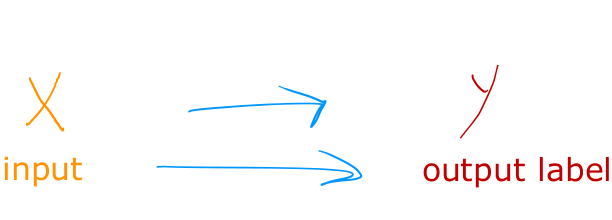
\includegraphics[width=0.8\textwidth]{figure/image.png}
    \caption{Cara Kerja Supervised Learning}
    \label{fig:2.carasupervised}
\end{figure}
\textit{Supervised learning} dibagi menjadi dua ranah dalam \textit{machine learning} yaitu klasifikasi dan regresi\cite{cunningham2008supervised}. Algoritma Klasifikasi digunakan untuk membuat prediksi berdasarkan kategori yang ditentukan yang artinya memiliki jumlah kemungkinan \textit{output} yang kecil, contohnya algoritma untuk memprediksi penipuan kartu kredit karena mengklasifikasi 2 kemungkinan yaitu transaksi penipuan dan transaksi normal \cite{cunningham2008supervised}. Algoritma Regresi merupakan sebuah algoritma yang mendeteksi nilai yang berkelanjutan, contohnya seperti sistem prediksi kenaikan harga saham karena memungkinkan untuk memiliki banyak kemungkinan \textit{output} untuk mengetahui hasil prediksinya\cite{cunningham2008supervised}. 


\subsection{\textit{Gradient Descent}} \label{II.Gradient Descent}
\textit{Gradient descent} merupakan sebuah \textit{optimization algorithm} yang umum digunakan untuk melatih model \textit{machine learning} dan \textit{neural networks}\cite{hochreiter2001learning}. \textit{Gradient descent} melatih \textit{machine learning} models dengan minimalisasi errors antara hasil prediksi dan nilai asli dengan mengganti parameter w dan b\cite{hochreiter2001learning}.

\textit{Cost function} merupakan cara untuk mengetahui performa dari sebuah model, dengan cara mengurang \textit{output} hasil prediksi dengan hasil sebenarnya untuk mendapatkan nilai akurasi, semakin kecil keluaran nilai dari \textit{cost function} maka akurasi semakin baik\cite{alpaydin2021machine}. Contohn dalam model \textit{linear regression} yang mempunyai rumus untuk modelnya dalam bentuk seperti ini  $y = wx + b$ yang mana $y = f_{w,b}(x)$ maka formula dari cost function menjadi seperti ini.\\
\begin{equation}
    J(w,b) = \frac{1}{2m} \sum\limits_{i = 0}^{m-1} (f_{w,b}(x^{(i)}) - y^{(i)})^2
\end{equation}
\label{eq:2.CostFunction}
\myequations{Rumus Cost Function}
\\
dengan diketahui bahwa:
\begin{center}
$J(w,b)$ = \textit{cost function} dengan parameter w dan b\\
$w$ = slope / turunan\\
$b$ = \textit{y-axis intercept}\\
$m$ = jumlah data training\\
$y$ = nilai sebenarnya\\
$f_w,_b$ = nilai prediksi\\
$i$ = nilai iterasi\\
\end{center}

\subsubsection{Perhitungan \textit{Cost Function}} \label{II.costfunction}
Perhitungan \textit{cost function} untuk membuat sebuah model prediksi \textit{linear regression} dengan dataset sederhana dengan jumlah 2 data dengan fitur x dan y. Data pertama x = 1 dan y = 300 dan data kedua x = 2 dan y = 500.

Perhitungan cost function digunakan untuk mengetahui gambaran performa dari sebuah model dengan inputan w dan b tertentu. Contoh inputkan w = 150, b = 100 dan nilai x yang di inputkan ke dalam sebuah model \textit{linear regression} $y = wx + b$ dan setelah itu hitung cost functionnya.

Hasil dari \textit{cost function} w = 150 dan b = 100 adalah 3.125 yang tergambarkan dengan grafik \textit{scatter plot} untuk y dan x seperti pada gambar \ref{fig:2.scatterplotlinear}.
\begin{figure}[H] % Kalau menggunakan H, posisi gambar akan tepat dibawah teks
    \centering
    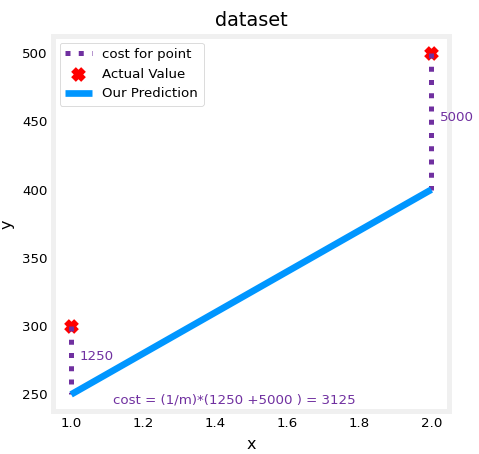
\includegraphics[width=0.5\textwidth]{figure/scatter plot linear regression.png}
    \caption{Scatter Plot Linear Regression}
    \label{fig:2.scatterplotlinear}
\end{figure}
Grafik \textit{scatter plot} tersebut menunjukan bahwa hasil \textit{cost function} w = 150 dan b = 100 belum menghasilkan \textit{output} yang baik dikarenakan \textit{straight line} belum \textit{fit} kedalam data dan bisa dilihat pada gambar \ref{fig:2.scatterplotcost} dan nilai w yang belum mencapai nilai \textit{local minimum}.
\begin{figure}[H] % Kalau menggunakan H, posisi gambar akan tepat dibawah teks
    \centering
    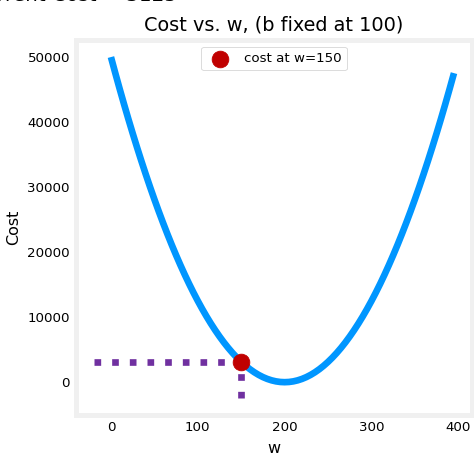
\includegraphics[width=0.5\textwidth]{figure/Scatter plot cost function.png}
    \caption{Scatter Plot Cost Function}
    \label{fig:2.scatterplotcost}
\end{figure}

\subsubsection{Cara Kerja \textit{Gradient Descent}} \label{II.carakerjagradientdescent}
\textit{Gradient descent} merupakan algoritma yang digunakan untuk terus mengubah w dan b untuk mengurangi $j(w,b)$ sampai akhirnya mencapai \textit{local minimum}\cite{hochreiter2001learning}. Analoginya ialah seperti pendaki yang ingin turun bukit namun banyak kabut disekitarnya sehingga dia tidak bisa melihat contohnya seperti pada gambar \ref{fig:2.gradientdescent}.
\begin{figure}[H] % Kalau menggunakan H, posisi gambar akan tepat dibawah teks
    \centering
    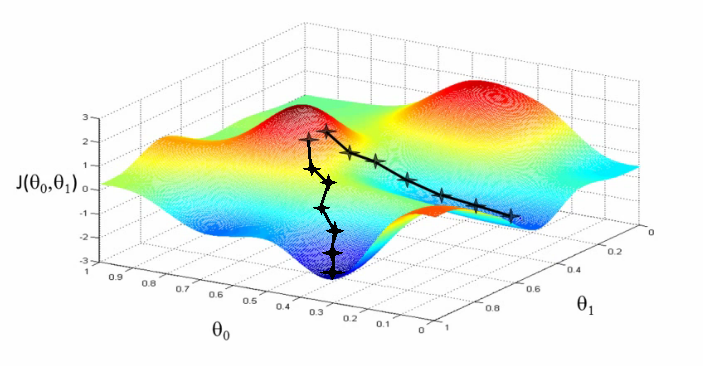
\includegraphics[width=0.5\textwidth]{figure/gradient descent.png}
    \caption{Gradient Descent}
    \label{fig:2.gradientdescent}
\end{figure}
Seperti yang terlihat pada gambar \ref{fig:2.gradientdescent}. pendaki akan mencoba untuk mencari cara untuk turun ke dasar dengan cara mengecek sekelilingnya dan setelah itu mencoba untuk melangkah satu kali dan setelah itu mengecek apakah langkah tersebut membuatnya turun atau tidak, jika turun maka pendaki akan mencoba untuk melangkah ke arah yang sama dan jika tidak maka pendaki mencoba langkah yang berbeda dan ada hal perlu diperhatikan pada gambar \ref{fig:2.gradientdescent} yang menunjukan bahwa local minimum bisa terdapat lebih dari 1\cite{ruder2016overview}.

Gradient descent memiliki formula seperti cost function untuk menjalankan sebuah algoritma nya untuk mengganti nilai w dan b agar bisa mencapai \textit{local minimum}.\\
Formula gradient descent\cite{ruder2016overview}: \\
\begin{equation}
\text{repeat until convergence: } 
\left\lbrace
\begin{aligned}
  w &= w - \alpha \frac{\partial J(w,b)}{\partial w} \\
  b &= b - \alpha \frac{\partial J(w,b)}{\partial b}
\end{aligned}
\right.
\end{equation}
\label{eq:2.gradient}
\myequations{Rumus Gradient Descent}
\\
yang diketahui bahwa:
\begin{center}
    $\alpha$ = \textit{Learning rate}\\
    $\partial$ = \textit{Partial derivative}
\end{center}
Yang mana parameter w dan b akan \textit{update simultaneously}.\\
Hasil dari \textit{partial derivative} dari $\frac{\partial J(w,b)}{\partial w}$ dan juga $\frac{\partial J(w,b)}{\partial b}$ seperti berikut. \\
\begin{equation}
    \begin{aligned}
    \frac{\partial J(w,b)}{\partial w} &= \frac{1}{m} \sum_{i=0}^{m-1} \left( f_{w,b}\left(x^{(i)}\right) - y^{(i)} \right) x^{(i)} \\
    \frac{\partial J(w,b)}{\partial b} &= \frac{1}{m} \sum_{i=0}^{m-1} \left( f_{w,b}\left(x^{(i)}\right) - y^{(i)} \right)
    \end{aligned}
\end{equation}
\label{eq:2.partialgradient}
\myequations{Hasil Partial Derivative Gradient}

\subsubsection{Learning Rate} \label{II.learningrate}
Learning Rate($\alpha$) merupakan salah satu parameter terpenting dalam \textit{machine learning} terkhusus dalam konteks \textit{gradient descent}\cite{igiri2015effect}. \textit{ Learning rate} menentukan ukuran langkah yang dapat diambil pada setiap iterasinya\cite{zeiler2012adadelta}. Menentukan \textit{learning rate} merupakan hal yang krusial dikarenakan jika \textit{learning rate} terlalu kecil maka gradient descent akan berjalan sangat lambat seperti pada gambar \ref{fig:2.learningratekecil} dan apabila nilai learning rate terlalu besar maka bisa terjadi \textit{overshoot} atau tidak pernah mencapai \textit{local minimum} seperti pada gambar \ref{fig:2.learningratebesar}\cite{igiri2015effect}.
\begin{figure}[H] % Kalau menggunakan H, posisi gambar akan tepat dibawah teks
    \centering
    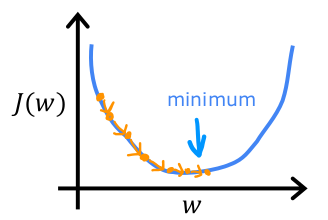
\includegraphics[width=0.5\textwidth]{figure/Learning rate kecil.png}
    \caption{Learning Rate Terlalu Kecil}
    \label{fig:2.learningratekecil}
\end{figure}
\begin{figure}[H] % Kalau menggunakan H, posisi gambar akan tepat dibawah teks
    \centering
    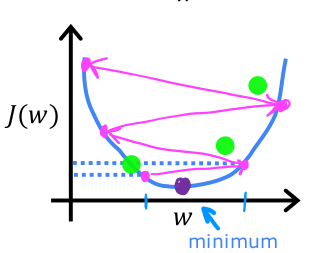
\includegraphics[width=0.5\textwidth]{figure/Learning rate besar.png}
    \caption{Learning Rate Terlalu Besar}
    \label{fig:2.learningratebesar}
\end{figure}
Ada berbagai cara untuk menentukan nilai learning rate terbaik salah satu cara paling umum dilakukan ialah dengan menggunakan \textit{grid search}, dengan \textit{grid search} kita bisa melakukan berbagai iterasi dengan nilai learning rate berbeda-beda dan lakukan analsis komparasi untuk menentukan nilai \textit{learning rate} terbaik\cite{smith2018disciplined}. Salah satu cara untuk memilih range nilai learning rate yang akan dimasukan ke grid search ialah dengan skala logaritmic contohnya dari $10^{-6}$ sampai $10^{-1}$\cite{smith2018disciplined}.


\subsection{Kartu Kredit} \label{II.KartuKredit}
Kartu kredit merupakan alat pembayaran nontunai yang memberikan fasilitas kredit kepada pemegang nya\cite{wooster1966credit}. Pemegang kartu kredit wajib membayar tagihan  akibat penggunaan kartu tersebut pada waktu yang  ditentukan dalam kontrak\cite{wooster1966credit}. Kewajiban pembayaran ini berlaku untuk seluruh transaksi yang dilakukan, termasuk pembelian barang dan jasa serta penarikan uang tunai\cite{flitcroft2009credit}. 

Ada dua jenis transaksi  kartu kredit: transaksi \textit{card-present}(CP) dan transaksi \textit{card-not-present}(CNP)\cite{kumar2016method}. Transaksi \textit{card-present} terjadi ketika kartu kredit secara fisik digunakan di lokasi transaksi, misalnya saat berbelanja di toko dan menggesek kartu di mesin EDC. Sebaliknya, transaksi \textit{card-not-present} tidak memerlukan kehadiran fisik kartu, seperti saat berbelanja online atau melakukan pembayaran melalui telepon dan dalam transaksi CNP, data kartu kredit dimasukkan secara manual atau otomatis ke dalam sistem pembayaran\cite{kumar2016method}. Berikut merupakan contoh bagian-bagian yang ada pada sebuah kartu kredit.
\begin{enumerate}[noitemsep]
    \item \textit{Chip}  kartu kredit terletak di bagian depan kartu. \textit{Chip} ini ditambahkan pada berbagai aplikasi yang dapat mengenkripsi data agar dapat disimpan dengan lebih aman.
    \item  Nomor kartu adalah 16 digit nomor kartu kredit. Nomor ini tidak akan pernah sama dengan nomor kartu kredit lainnya.
    \item \textit{Cardholder Name} adalah nama  pemilik atau pemegang kartu kredit.
    \item Nama atau logo penerbit adalah nama atau logo perusahaan penerbit kartu.
    \item Masa berlaku adalah tanggal dalam format dua digit setelah bulan dan tahun  masa berlaku kartu kredit.
    \item Logo jaringan kartu (GPN pada diagram) adalah logo jaringan kartu kredit.
    \item Terdapat strip magnet di bagian belakang yang dapat dibaca dengan menggesek kartu saat bertransaksi.
    \item Tanda tangan pemegang kartu dimasukkan pada kolom tanda tangan.
    \item  Nomor verifikasi atau CVV/CVC adalah 3 digit angka di sebelah kolom tanda tangan.
    \item Alamat bank penerbit adalah alamat perusahaan/bank yang menerbitkan kartu.
    \item  Nama atau logo penerbit kartu.
\end{enumerate}
\begin{figure}[H] % Kalau menggunakan H, posisi gambar akan tepat dibawah teks
    \centering
    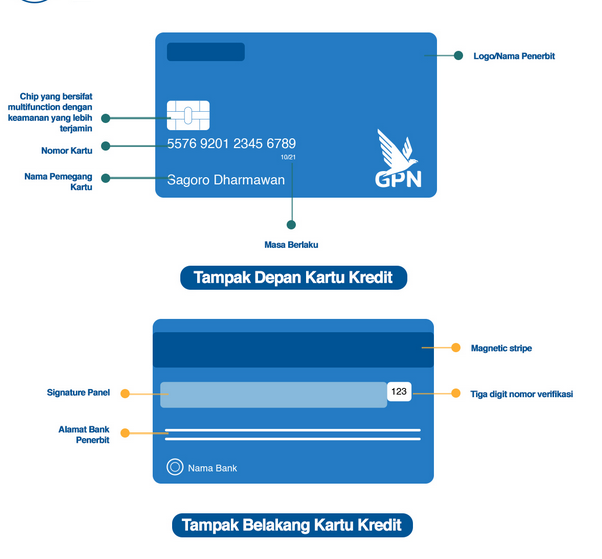
\includegraphics[width=0.5\textwidth]{figure/kartu.png}
    \caption{Kartu Kredit}
    \label{fig:2.kartukredit}
\end{figure}

\subsection{\textit{Imbalanced data}} \label{II.Imbalanced Data}
\textit{Imbalanced data} merupakan sebuah kondisi di sebuah data di mana jumlah data antara kelas satu dan lainnya tidak seimbang yang artinya salah satu kelas memiliki jumlah yang lebih besar dibandingkan lainnya\cite{haixiang2017learning}. \textit{Imbalanced dataset} kemunculannya merupakan hal alami yang akan selalu muncul pada kejadian yang langka, namun kejadian langka tersebut bisa menyebabkan hal buruk apabila terjadi, salah satu contohnya ialah  pada data transaksi penipuan, data penyakit kanker\cite{krawczyk2016learning}. Kejadian langka tersebut dapat mengakibatkan kerugian besar apabila terjadi dan dibutuhkan sistem yang bisa memprediksi kejadian langka tersebut\cite{krawczyk2016learning}.

\textit{Imbalanced dataset} merupakan masalah yang besar di sebuah\textit{ machine learning} dikarenakan dapat mengakitbatkan bias yang cenderung lebih ke kelas mayoritas. hal ini membuat model menjadi sulit untuk mendeteksi kelas dengan jumlah lebih sedikit atau minoritas\cite{haixiang2017learning}. Berikut ini merupakan visualisasi \textit{imbalanced data} yang dapat dilihat pada gambar \ref{fig:2.visualisasiimbalanced}.
\begin{figure}[H] % Kalau menggunakan H, posisi gambar akan tepat dibawah teks
    \centering
    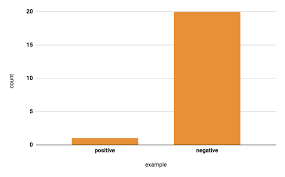
\includegraphics[width=0.5\textwidth]{figure/gambar imbalance data.png}
    \caption{Visualisasi Imbalanced Data}
    \label{fig:2.visualisasiimbalanced}
\end{figure}

\subsection{\textit{Hyperparameter}} \label{II.hyperparameter}
\textit{Hyperparameter} adalah parameter yang ditentukan sebelum proses pelatihan model pembelajaran mesin dimulai\cite{yang2020hyperparameter}. Berbeda dengan parameter model, yang dipelajari secara otomatis selama pelatihan, \textit{hyperparameter} memengaruhi cara model mempelajari dan mengambil keputusan\cite{bischl2023hyperparameter}. Contoh \textit{hyperparameter} ialah:
\begin{enumerate}[noitemsep]
    \item \textit{Learning rate}.
    \item jumlah iterasi.
    \item jumlah \textit{tree} dalam \textit{ensemble methods}.
    \item kedalaman \textit{tree} dalam \textit{decision tree}.
    \item jumlah \textit{neuron} dalam \textit{neural network}.
\end{enumerate}
\textit{Hyperparameter} berguna dalam membangun strutur dan kompleksitas dari model \textit{machine learning}. Pemilihan \textit{hyperparameter} yang tepat dapat sangat mempengaruhi kinerja model\cite{bischl2023hyperparameter}. Cara menentukan \textit{hyperparameter} bisa dilakukan dengan berbagai cara seperti berikut ini.\cite{yang2020hyperparameter}:
\begin{enumerate}[noitemsep]
    \item \textit{Grid Search}
    \item \textit{Random Search}
    \item \textit{Bayesian Optimization}
    \item \textit{Manual Tuning}
    \item \textit{Automated Hyperparameter Tuning(seperti Optuna)}
\end{enumerate}

\subsection{Feature Engineering} \label{II.featureengineering}
\textit{Feature engineering} adalah proses penting dalam \textit{machine learning} yang melibatkan pemilihan, modifikasi, atau penciptaan fitur (variabel input) yang membantu sebuah model untuk belajar\cite{alpaydin2021machine}. Tujuan dari \textit{feature engineering} adalah untuk meningkatkan performa model dengan menyediakan representasi data yang lebih baik\cite{alpaydin2021machine}.   

\subsubsection{Feature Creation} \label{II.featurecreation}
Feature creation merupakan salah satu tipe \textit{feature engineering} yang mana fitur-fitur atau variabel-variabel baru diciptakan berdasarkan data yang sudah ada\cite{alpaydin2021machine}. Tujuannya adalah untuk menyediakan informasi tambahan yang mungkin tidak langsung tersedia dalam data mentah, tetapi bisa membantu model pembelajaran mesin dalam membuat prediksi yang lebih akurat\cite{dong2018feature}. Salah satu contoh kegunaan dari feature creation adalah dalam mengenali sebuah ciri-ciri tertentu yang digunakan untuk membuat sistem prediksi, seperti ingin prediksi harga sebuah rumah berdasarkan data panjang dan lebar, dengan data tersebut kita bisa membuat fitur baru seperti luas dengan mengalikan panjang dan lebar. Contoh visualisasi dalam kasus ini ialah saat kita memiliki data yang memiliki fitur panjang dan lebar dan mencoba untuk dimasukan kedalam sebuah model machine learning dan ternyata hasil dari model machine learning belum bisa dikatakan baik seperti pada gambar \ref{fig:2.visualisasisebelumfeaturecreation}. Dalam hal ini kita mungkin harus mencoba membuat feature creation baru agar dapat menghasilkan hasil model machine learning yang lebih baik dengan membuat feature creation luas dan ternyata hasil dari machine learning menjadi lebih baik seperti pada gambar \ref{fig:2.visualisasisesudahfeaturecreation}.

\begin{figure}[H] % Kalau menggunakan H, posisi gambar akan tepat dibawah teks
    \centering
    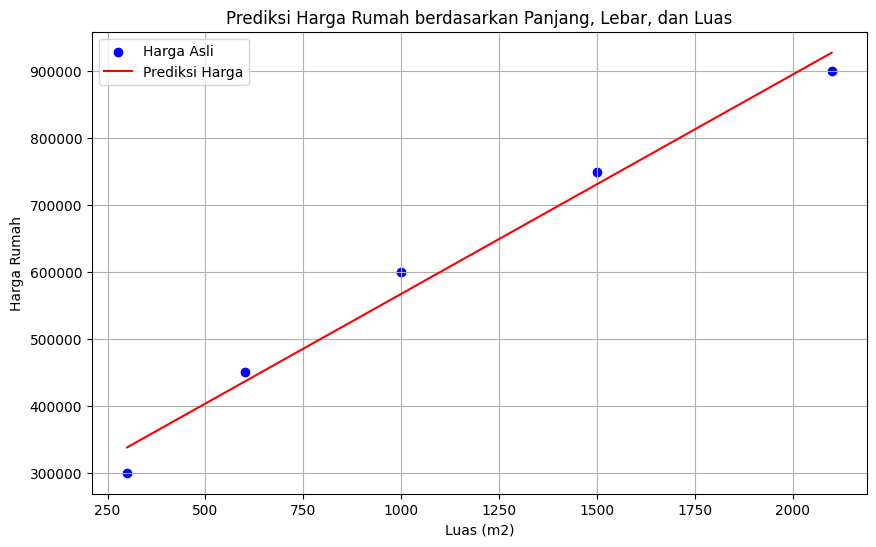
\includegraphics[width=0.5\textwidth]{figure/output feature creation only one feature.png}
    \caption{Visualisasi Sebelum Feature Creation}
    \label{fig:2.visualisasisebelumfeaturecreation}
\end{figure}

\begin{figure}[H] % Kalau menggunakan H, posisi gambar akan tepat dibawah teks
    \centering
    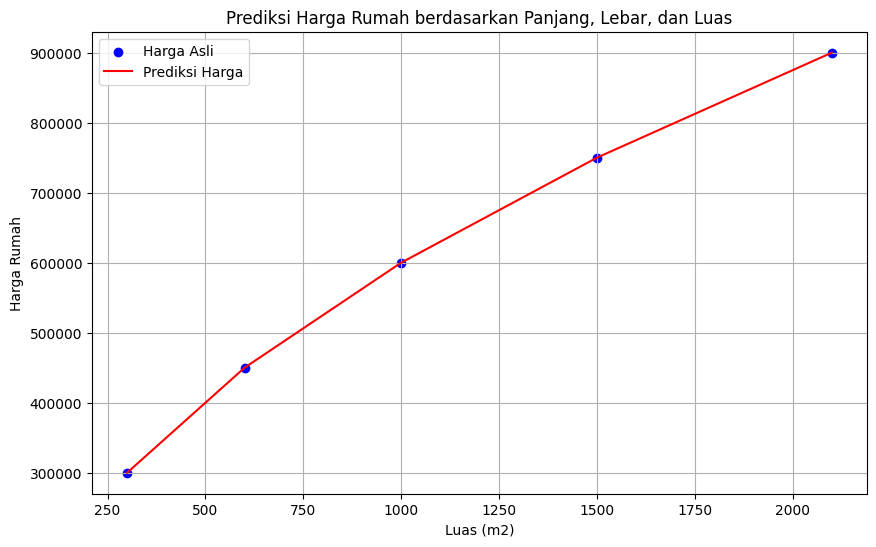
\includegraphics[width=0.5\textwidth]{figure/output feature creation multiple feature.png}
    \caption{Visualisasi Sesudah Feature Creation}
    \label{fig:2.visualisasisesudahfeaturecreation}
\end{figure}
Hasil dari visualiasi diatas menunjukan kalau feature creation dapat meningkatkan kemampuan model dalam belajar namun setelah mengetahui hal tersebut diperlukan pertimbangan agar tidak terjadi overfitting saat melakukan feature creation.

\subsubsection{Feature Scaling} \label{II.featurescaling}
\textit{Feature scaling} adalah sebuah proses untuk mengubah rentang nilai fitur dalam sebuah \textit{dataset} menjadi seimbang atau dengan skala yang sama\cite{alpaydin2021machine}. Hasil proses \textit{feature scaling} sangat penting dalam \textit{machine learning} dikarenakan untuk menghindari sensitivitas dalam algoritma yang membuat ada sebuah fitur mendominasi fitur lainnnya\cite{dong2018feature}. Feature Scaling juga mempengaruhi bagaimana algoritma \textit{gradient descent} bekerja, dengan memiliki skala yang tidak seimbang maka akan membuat \textit{gradient descent} menjadi lebih lama dalam menemukan \textit{local minimum} atau bahkan tidak menemukannya sama sekali\cite{ruder2016overview}. Cara melakukan \textit{feature scaling} dalam python ialah dengan menggunakan \textit{library} \textit{scikit-learn} terkait \textit{preprocessing}. Hasil dari \textit{feature scaling} ialah membuat rentang nilai antara fitur satu dan lainnya menjadi lebih setara seperti pada gambar \ref{fig:2.visualisasisebelumfeaturescaling} menunjukan bahwa fitur 2 dan fitur 3 mempunyai rentang nilai yang sangat berbeda, dan setelah melakukan \textit{feature scaling} seperti pada gambar \ref{fig:2.visualisasisesudahfeaturescaling} menunjukan bahwa rentang nilainya menjadi lebih seimbang.
\begin{figure}[H] % Kalau menggunakan H, posisi gambar akan tepat dibawah teks
    \centering
    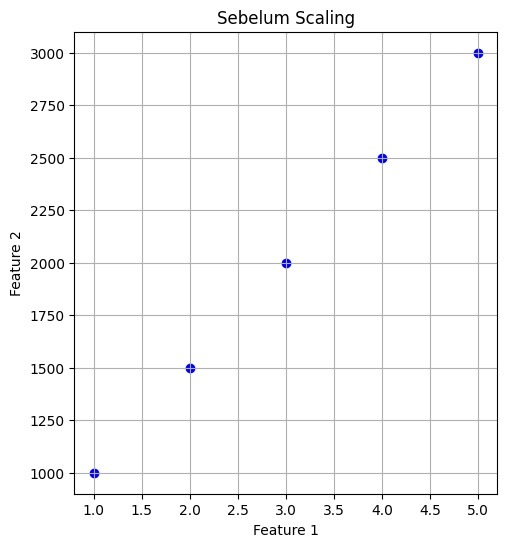
\includegraphics[width=0.5\textwidth]{figure/before feature scaling.png}
    \caption{Visualisasi Sebelum Feature Scaling}
    \label{fig:2.visualisasisebelumfeaturescaling}
\end{figure}
\begin{figure}[H] % Kalau menggunakan H, posisi gambar akan tepat dibawah teks
    \centering
    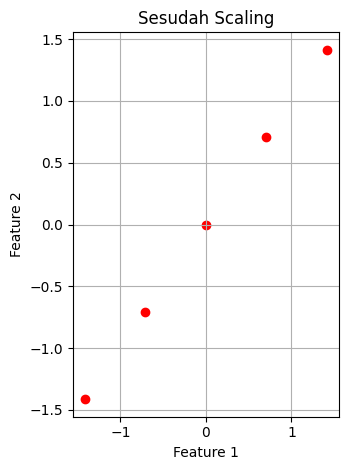
\includegraphics[width=0.5\textwidth]{figure/after feature scaling.png}
    \caption{Visualisasi Sesudah Feature Scaling}
    \label{fig:2.visualisasisesudahfeaturescaling}
\end{figure}
Dari contoh diatas dapat dilihat bahwa rentang nilai dari fitur satu dan fitur dua menjadi lebih seimbang yang artinya membuat machine learning untuk belajar dengan hasil yang lebih baik

\subsection{\textit{Oversampling}} \label{II.oversampling}
\textit{Oversampling} adalah teknik yang digunakan dalam \textit{machine learning} dan analisis data untuk menangani masalah \textit{unbalanced} data dalam dataset\cite{liu2004effect}. \textit{Unbalanced data} muncul ketika terdapat satu kelas atau fitur yang memiliki jumlah data sampel yang jauh lebih banyak dibandingkan kelas atau fitur lainnya\cite{dal2015calibrating}. Contohnya, dalam \textit{dataset} untuk mendeteksi penipuan kartu kredit, total jumlah transaksi yang normal mungkin jauh lebih banyak daripada jumlah transaksi penipuan.

Tujuan dari \textit{oversampling} ialah untuk membuat data menjadi \textit{balance} atau seimbang agar saat diinputkan ke \textit{machine learning}, model tidak menjadi bias terhadap kelas mayoritas. Salah satu contoh dari metode \textit{oversampling ialah} SMOTE\cite{chawla2002smote} dan ADASYN\cite{4633969}.   

\subsection{SMOTE (Synthetic Minority Over-sampling Technique)} \label{III.smote}
SMOTE atau bisa disebut \textit{Synthetic Minority Over-sampling technique} adalah sebuah metode yang digunakan untuk mengatasi masalah ketidaksemibangan (imbalance) kelas dalam dataset\cite{chawla2002smote}. SMOTE digunakan untuk tugas klasifikasi. SMOTE bekerja dengan membuat sampel sintetis dari kelas minoritas untuk meningkatkan jumlah sampel kelas minoritas sehingga dataset menjadi lebih seimbang dengan kelas mayoritas\cite{chawla2002smote}. SMOTE tidak menduplikasi sample yang sudah ada tapi SMOTE menghasilkan sampel baru dengan interpolasi sample minoritas\cite{chawla2002smote}.
\subsubsection{Cara Kerja SMOTE}
Berikut cara kerja dibalik SMOTE:
\begin{enumerate}[noitemsep]
    \item Pemilihan sampel pada fitur minoritas dengan contohnya sampel x pada suatu fitur minoritas
    \item Cari \textit{k-nearest neighbors}          (tetangga terdekat) dari sampel x didalam fitur minoritas.
    \item Pilih secara acak salah satu dari \textit{k-nearest neighbors} yang kita sebut sebagai $x_{neighbor}$
    \item Buat sampel baru dengan linear interpolasi antara sampel x dan $x_{neighbor}$ yang kita sebut $x_{synthetic}$ dengan perhitungan sebagai berikut:\\
    
    \begin{equation}
    x_{synthetic} = x + \lambda . (x_{neighbor} - x)   
    \end{equation}\\
    \label{eq:2.smote}
    \myequations{Rumus membuat data sintetis}
    yang mana $\lambda$ merupakan bilangan acak antara 0 dan 1.
\end{enumerate}
Hasil dari metode oversampling SMOTE akan menghasilkan pola data yang sebelumnya merupakan seperti ini pada gambar \ref{fig:2.visualisasidatasebelumsmote} menjadi seperti ini pada gambar \ref{fig:2.visualisasidatasesudahsmote}. Pada gambar \ref{fig:2.visualisasidatasesudahsmote} dapat dilihat kalau metode oversampling SMOTE membuat data sample berdasarkan pola dari data sebelumnya dengan membuat garis interpolasi antar data poin terdekatnya yang mana menghasilkan data sintetis yang bnyk namun sama dengan pola data sebelumnya.
\begin{figure}[H]
	\centering
	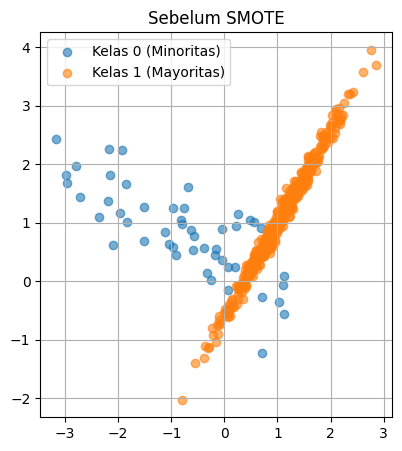
\includegraphics[width=0.5\textwidth]{figure/visualisasi_data_sebelum_smote.png}
	\caption{Visualisasi Data Sebelum SMOTE}
	\label{fig:2.visualisasidatasebelumsmote}
\end{figure}

\begin{figure}[H]
	\centering
	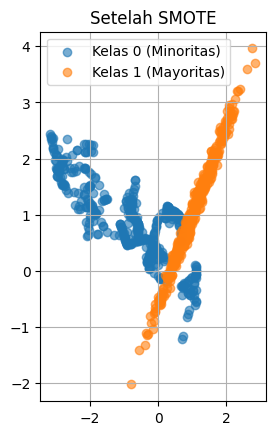
\includegraphics[width=0.5\textwidth]{figure/visualisasi_data_sesudah_smote.png}
	\caption{Visualisasi Data Sesudah SMOTE}
	\label{fig:2.visualisasidatasesudahsmote}
\end{figure}

\subsection{ADASYN (Adaptive Synthetic Sampling)} \label{II.adasyn}
ADASYN (\textit{Adaptive Synthetic Sampling}) adalah teknik yang digunakan untuk menangani ketidakseimbangan(imbalance) kelas dalam tugas klasifikasi, namun dengan pendekatan yang lebih adaptif dibandingkan metode seperti SMOTE\cite{4633969}. ADASYN bekerja dengan membuat sampel sintetis baru untuk kelas minoritas. ADASYN berfokus pada sampel yang sulit untuk diklasifikasikan yang terletak di dekat perbatasan antara kelas mayoritas dan minoritas\cite{4633969}.
\subsubsection{Cara kerja ADASYN}
Berikut cara kerja dibalik ADASYN:
\begin{enumerate}[noitemsep]
    \item Yang pertama ialah tentukan jumlah sampel sintetis yang perlu dibuat untuk setiap sampel minoritas $x_i$ berdasarkan tingkat kesulitan klasifikasi lokal. Tingkat kesulitan lokal $d_i$ dihitung berdasarkan jumlah tetangga terdekat dari kelas mayoritas di sekitar $x_i$.
    \item Yang kedua hitung bobot adaptif atau $r_i$ untuk setiap sampel minoritas $x_i$\\
    yang mana $n_{min}$ adalah jumlah sampel kelas minoritas. Menghitung bobot adaptif ini digunakan untuk menentukan seberapa banyak sampel sintetis yang perlu dibuat untuk setiap sampel minoritas.
    \item Yang terakhir ialah membuat sampel sintetis berdasarkan jumlah total sampel sintetis yang diinginkan. sampel sintetis dibuat dengan menggunakan rumus interpolasi linear SMOTE seperti pada rumus 2.4.\\
\end{enumerate}
Hasil dari metode oversampling ADASYN akan menghasilkan pola data yang berbeda dengan sebelumnya seperti pada gambar \ref{fig:2.visualisasidatasebelumadasyn} menjadi seperti ini pada gambar \ref{fig:2.visualisasidatasesudahadasyn}. Pada gambar \ref{fig:2.visualisasidatasesudahadasyn} dapat dilihat kalau metode oversampling ADASYN membuat data sintetis berdasarkan bobot yang sudah ditentukan sebelumnya dan setalh itu membuat garis interpolasi antar data poin terdekatnya yang mana menghasilkan data sintetis yang banyak namun memiliki data yang cenderung berkumpul pada pertemuan antara data minortas dan mayoritas.

\begin{figure}[H]
	\centering
	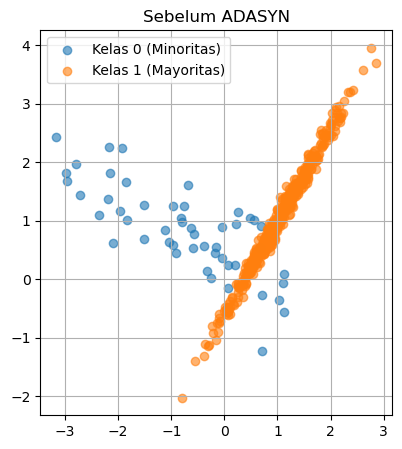
\includegraphics[width=0.5\textwidth]{figure/visualisasi_data_sebelum_adasyn.png}
	\caption{Visualisasi Data Sebelum ADASYN}
	\label{fig:2.visualisasidatasebelumadasyn}
\end{figure}

\begin{figure}[H]
	\centering
	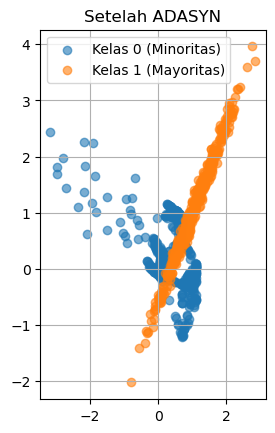
\includegraphics[width=0.5\textwidth]{figure/visualisasi_data_sesudah_adasyn.png}
	\caption{Visualisasi Data Sesudah ADASYN}
	\label{fig:2.visualisasidatasesudahadasyn}
\end{figure}

\subsection{\textit{Decision Tree}} \label{II.decisiontree}
\textit{Decision Tree} merupakan sebuah algoritma machine learning yang digunakan untuk tugas klasifikasi dan regresi dengan memprediksi berdasarkan serangkaian kondisi atau pertanyaan tertentu\cite{song2015decision}. \textit{Decision Tree} sering di visualisasikan dengan gambar pohon terbaik dengan bagian paling atas disebut \textit{root node} dan setiap \textit{node} dibawah \textit{root node} yang ditunjuk oleh panah dan menunjuk panah bisa disebut dengan \textit{decision node atau branches} dan untuk \textit{node} yang hanya ditunjuk dan tidak menunjuk \textit{node} disebut \textit{leaf node}\cite{rojas2012graphical}. Visualisasinya dapat dilihat pada gambar \ref{fig:2.decisiontree}.\\
\begin{figure}[H]
	\centering
	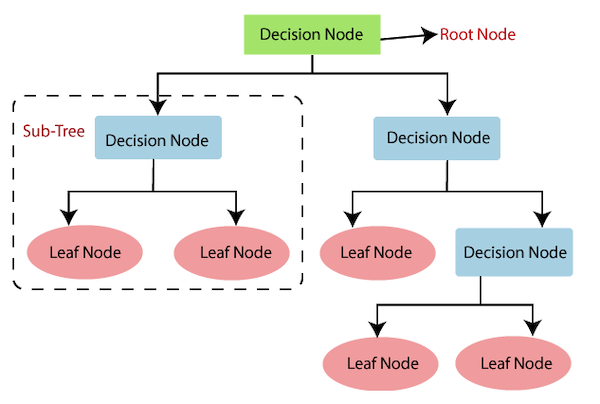
\includegraphics[width=0.5\textwidth]{figure/decision tree.png}
	\caption{Decision Tree}
	\label{fig:2.decisiontree}
\end{figure}
Cara \textit{decision tree} membuat keputusan ialah dengan dengan melakukan perhitungan pada setiap node nya untuk melanjutkan keputusan dengan cara menghitung \textit{gini impurity}, impurity berarti dalam \textit{decision tree} merupakan campuran dari keputusan iya atau tidak dan setelah menghitung gini impurity pada setiap keputusan iya dan tidak, kita hitung \textit{total gini impurity} untuk menjadi ukuran kualitas dari prediksi\cite{suthaharan2016decision}.\\ 
Berikut merupakan rumus \textit{gini impurity}:\\
\begin{equation} 
Gini(D) = 1 - \sum_{i=1}^k [p(i)]^2
\end{equation}
\label{eq:2.gini}
\myequations{Rumus Gini Impurity}\\
Yang dapat kita ketahui bahwa:\\
$D$ = merupakan node.\\
$k$ = merupakan jumlah kelas\\
$p(i)$ = merupakan peluang sampel yang termasuk kelas i pada node.\\
Berikut merupakan rumus dari \textit{total gini impurity}:\\ 
\begin{equation}
Total \ Gini \ Impurity = \sum_{i=1}^n \left[\frac{|D_i|}{|D|} \cdot Gini(D_i)\right]
\end{equation}
\label{eq:2.totalgini}
\myequations{Rumus Total Gini Impurity}\\
Yang mana dapat kita ketahui bahwa:\\
$n$ = merupakan jumlah \textit{node} pada sebuah \textit{tree}\\
$D_i$ = merupakan \textit{dataset} pada \textit{node} i\\
$D$ = merupakan  jumlah total sampel dalam \textit{dataset}\\

\subsection{Random Forest} \label{II.randomforest}
\textit{Random Forest} merupakan algoritma yang dibuat oleh Leo Breiman  yang mana pembuatan random forest ini merupakan lanjutan dari ide paper dia sebelumnya terkait bagging\cite{breiman2001random,breiman1996bagging}.
\textit{Random forest} merupakan salah satu algoritma ensemble learning bertipe \textit{bagging} yang digunakan untuk klasifikasi dan regresi. Algoritma ini bekerja dengan menggabungkan beberapa \textit{decision tree} untuk menghasilkan model yang lebih baik dalam menghindari \textit{overfitting}\cite{breiman2001random}. Setiap tree dalam \textit{random forest} dilatih dengan menggunakan subset data yang berbeda yang kita sebut sebagai \textit{boostrapped dataset} yang mana cara kerjanya cukup sederhana hanya memilih secara acak data yang ada pada original dataset dengan aturan:
\begin{enumerate}[noitemsep]
    \item Saat pemilihan acak boleh memilih data yang sama yang artinya apabila saat memilih data secara acak itu terpilih data yang sama maka itu diperbolehkan.
    \item Ukuran dari \textit{boostrapped dataset} itu harus sama dengan original dataset.
\end{enumerate}
Setelah membuat \textit{boostrapped dataset} akan dilakukan pembuatan decision tree dengan menggunakan boostrapped dataset, dalam pembuatan decision tree kita perlu menentukan berapa \textit{max feature} yang kita pilih secara acak pada setiap \textit{split tree}.

setelah pembuatan tree selesai dilakukan maka kita mengulang proses tersebut hingga ratusan kali atau sesuai yang kita yang tentukan dan keputusan akhir dibuat dengan menggabungkan hasil dari semua \textit{tree} sepeti pada gambar \ref{fig:2.randomforest}.

\begin{figure}[H]
	\centering
	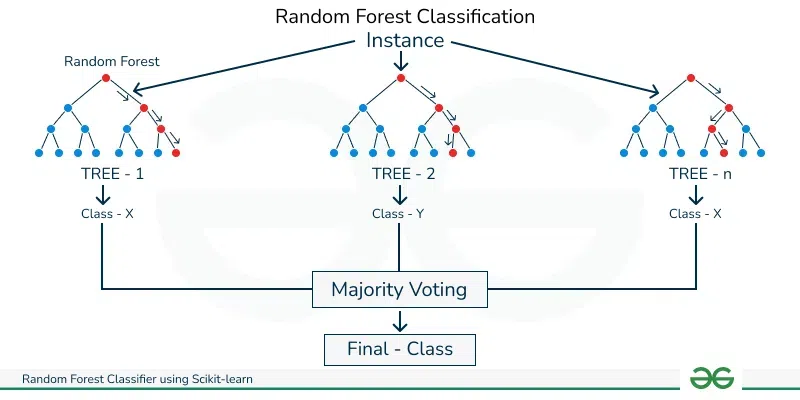
\includegraphics[width=0.7\textwidth]{figure/random_forest.png}
	\caption{Random Forest}
	\label{fig:2.randomforest}
\end{figure}
\textit{Random forest} memikiki banyak \textit{hyperparameter} yang digunakan untuk mengatur bagaimana random forest bekerja. \textit{Hyperparameter} yang digunakan dalam \textit{random forest} ialah sebagai berikut.
\begin{enumerate}[noitemsep]
    \item n\_estimator digunakan untuk menentukan seberapa banyak \textit{tree} yang ingin digunakan pada model \textit{random forest}.
    \item max\_depth digunakan untuk menentukan maksimum kedalaman \textit{tree}.
    \item min\_sample\_split digunakan untuk menentukan jumlah minimum yang dibutuhkan untuk \textit{split} pada \textit{internal node}.
    \item min\_sample\_leaf digunakan untuk menentukan jumlah \textit{minimum} yang dibutuhkan untuk membuat \textit{leaf node}.
    \item max\_feature digunakan untuk menentukan seberapa banyak \textit{feature} yang dibutuhkan pada setiap \textit{split}.
    \item bootstrap digunakan untuk menentukan apakah menggunakan \textit{boostrap sampling} atau tidak untuk membuat \textit{training set} pada setiap \textit{tree}.
\end{enumerate}

\subsection{XGBoost} \label{II.xgboost}
Extreme Gradient Boosting atau XGBoost adalah salah satu ensemble learning bertipe boosting dan merupakan sebuah algoritma \textit{machine learning} yang dioptimalkan untuk implementasi metode \textit{gradient boosting}\cite{chen2015xgboost}. Algoritma ini dikenal karena kecepatannya, efisiensinya, dan kemampuannya menghasilkan model yang sangat akurat, sehingga sering digunakan dalam kompetisi pembelajaran mesin seperti yang diadakan di platform Kaggle. \textit{XGBoost} digunakan untuk menyelesaikan masalah klasifikasi dan regresi\cite{chen2016xgboost}.

\textit{XGBoost} memikiki banyak \textit{hyperparameter} yang digunakan untuk mengatur bagaimana xgboost bekerja. \textit{Hyperparameter} yang digunakan dalam \textit{xgboost} ialah sebagai berikut\cite{xgboost_parameter_documentation}:
\begin{enumerate}[noitemsep]
    \item max\_depth digunakan untuk menentukan maksimum kedalaman \textit{tree}.
    \item learning\_rate digunakan untuk menentukan seberapa banyak step yang dilakukan pada setiap iterasi.
    \item n\_estimator digunakan untuk menentukan seberapa banyak tree yang ingin digunakan pada model xgboost.
    \item min\_child\_weight digunakan untuk menentukan jumlah bobot minimum yang digunakan dalam \textit{child node}.
    \item subsample digunakan untuk mengontrol seberapa banyak bagian \textit{training instances} yang digunakan pada setiap tree didalam xgboost.
    \item colsample\_bytree digunakan untuk mengontrol seberapa banyak \textit{feature} yang dipilih secara \textit{random sample} pada setiap \textit{tree} saat \textit{training}.
    \item gamma digunakan untuk menentukan minimum dari \textit{loss reduction} yang dibutuhkan untuk split \textit{tree}.
    \item alpha digunakan untuk mengontrol \textit{L1 regularization}.
\end{enumerate}

\subsection{Evaluasi Model} \label{II.evaluasimodel}
Pengujian model pada penelitian ini dengan membandingkan hasil test \textit{precision}, \textit{recall}, \textit{f1-score}, dan \textit{Matthews’s correlation coefficient} (MCC) \textit{metrics} untuk mendapatkan hasil terbaik. Untuk mendapatkan pengukuran tersebut dibutuhkan \textit{confusion matrix} seperti berikut.
\begin{figure}[H]
	\centering
	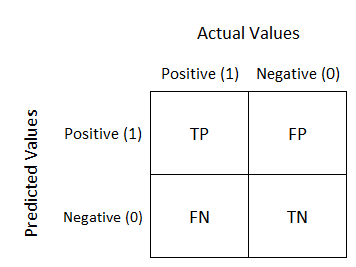
\includegraphics[width=0.5\textwidth]{figure/confusion_matrix.png}
	\caption{Confusion Matrix}
	\label{fig:2.confusionmatrix}
\end{figure}
yang mana \textit{confusion matrix} dibagi menjadi 4 yaitu:
\begin{enumerate}[noitemsep]
    \item True Positive (TP), jumlah data prediksi positif yang terdeteksi benar.
    \item True Negative (TN), jumlah data prediksi negatif yang terdeteksi benar.
    \item False Positive (FP), jumlah data prediksi negatif yang terdeteksi data positif.
    \item False Negative (FN), jumlah data prediksi positif yang terdeteksi data negatif.
\end{enumerate}
Barulah berdasarkan \textit{confusion matrix} kita dapat menghitung \textit{precision}, \textit{recall},     \textit{f-1 score}, dan \textit{Matthews’s correlation coefficient} (MCC) \textit{metrics}.

\subsubsection{Precision}
\textit{Precision} adalah perbandingan antara jumlah prediksi positif yang benar(TP) dengan total jumlah prediksi positif(TP + FP). \textit{Precision} menunjukan seberapa seberapa akurat model dalam memprediksi kelas positif. \textit{Precision} digunakan untuk menjawab pertanyaan seperti "dari semua \textit{instances} yang diprediksi positif, berapa banyak yang benar-benar positif?". \textit{Precision} dihitung dengan formula seperti berikut:\\
\begin{equation}
Precison = \frac{TP}{TP + FP} 
\end{equation}
\label{eq:2.precision}
\myequations{Rumus Precision}

Kegunaan dari \textit{precision} itu sangat penting dalam kasus dimana false positive tinggi. Contohnya dalam pendeteksi penipuan kartu kredit, kita ingin mengurangi kemungkinan mendeteksi transaksi yang tidak penipuan namun dikategorikan sebagai transaksi penipuan.
   
\subsubsection{Recall}
\textit{Recall} adalah perbandingan antara jumlah prediksi positif yang benar(TP) dengan total jumlah data aktual yang positif(TP+FN). \textit{Recall} menunjukkan seberapa baik model dalam menangkap semua data positif yang ada. \textit{Recall} digunakan untuk menjawab pertanyaan seperti "Dari semua kejadian yang benar-benar positif, berapa banyak yang diprediksi positif dengan tepat?". \textit{Recall} dapat dihitung dengan formula seperti berikut:\\
\begin{equation}
Precison = \frac{TP}{TP + FN} 
\end{equation}
\label{eq:2.recall}
\myequations{Rumus Recall}

Kegunaan dari \textit{recall} ialah pada kasus dimana memerlukan deteksi penyakit kita ingin recall yang tinggi untuk menangkap semua kasus penyakit agar tidak ada pasien yang tidak terdiagnosis. Recall berfokus pada  memastikan bahwa semua kasus positif terdekteksi meskipun ada beberapa kesalahan \textit{false positive} sedangkan \textit{precision} berguna ketika penting untuk memastikan bahwa prediksi benar-benar akurat, sehingga mengurangi jumlah \textit{false positive}.


\subsubsection{F1-Score}
\textit{F1-Score} adalah rata-rata harmonik dari precision dan recall. \textit{F1-Score} memberikan keseimbangan antara precision dan recall yang berguna saat ada ketidakseimbangan kelas.\\
\begin{equation}
F1-Score = 2 \times \frac{Precision \times Recall}{Precision + Recall}   
\end{equation}
\label{eq:2.f1score}
\myequations{Rumus F1 Score}

Kegunaan dari \textit{f1-score} ialah pada situasi dimana penting untuk menjaga keseimbangan antara \textit{precision} dan recall, untuk menghindari bias terhadap kelas mayoritas.    

\subsubsection{Matthews correlation coefficient}
\textit{Matthew’s Correlation Coefficient} 
(MCC) adalah ukuran evaluasi yang digunakan untuk mengukur kinerja sebuah model dalam melakukan klasifikasi biner. MCC berkerja dengan mempertimbangkan semuan nilai yang ada dalam \textit{confusion matrix}(TP, TN, FP, FN) dalam menggambarkan hasil kualitas prediksi model, dikarenakan mcc mempertimbangkan semua elemen yang ada pada confusion metrix maka mcc dapat dijadikan sebuah metrik evaluasi yang baik untuk kelas yang tidak seimbang(\textit{unbalance})\cite{chicco2020advantages}. MCC dapat dihitung dengan formula seperti berikut:\\
\begin{equation}
MCC = \frac{(TP \times TN) - (FP \times FN)}{\sqrt{(TP + FP)(TP + FN)(TN + FP)(TN + FN)}} 
\end{equation}
\label{eq:2.mcc}
\myequations{Rumus Matthews correlation coefficient}

Hasil dari nilai \textit{matthew's Correlation Coefficient} diinterpretasikan sebagai berikut.
\begin{enumerate}[noitemsep]
    \item +1: Model membuat prediksi sempurna (semua prediksi benar).
    \item 0: Model tidak bisa melakukan prediksi dan sama seperti tebakan acak.
    \item 1: Model membuat prediksi yang salah secara total.
\end{enumerate}

Pada penelitian ini juga peneliti akan menggunakan mcc sebagai metrik utama untuk menentukan gambaran performa model dan peneliti tidak akan menggunakan roc auc disebabkan semakin tinggi hasil dari mcc(contoh: MCC = 0.9) maka semakin tinggi pula nilai roc auc namun tidak sebaliknya\cite{chicco2023matthews}.



    \newpage
\chapter{Analisis dan Perancangan} \label{Bab III}

\section{Alur Penelitian} \label{III.Alur}
berikut merupakan alur penelitian yang dilakukan oleh peneliti.
\begin{figure}[H]
	\centering
	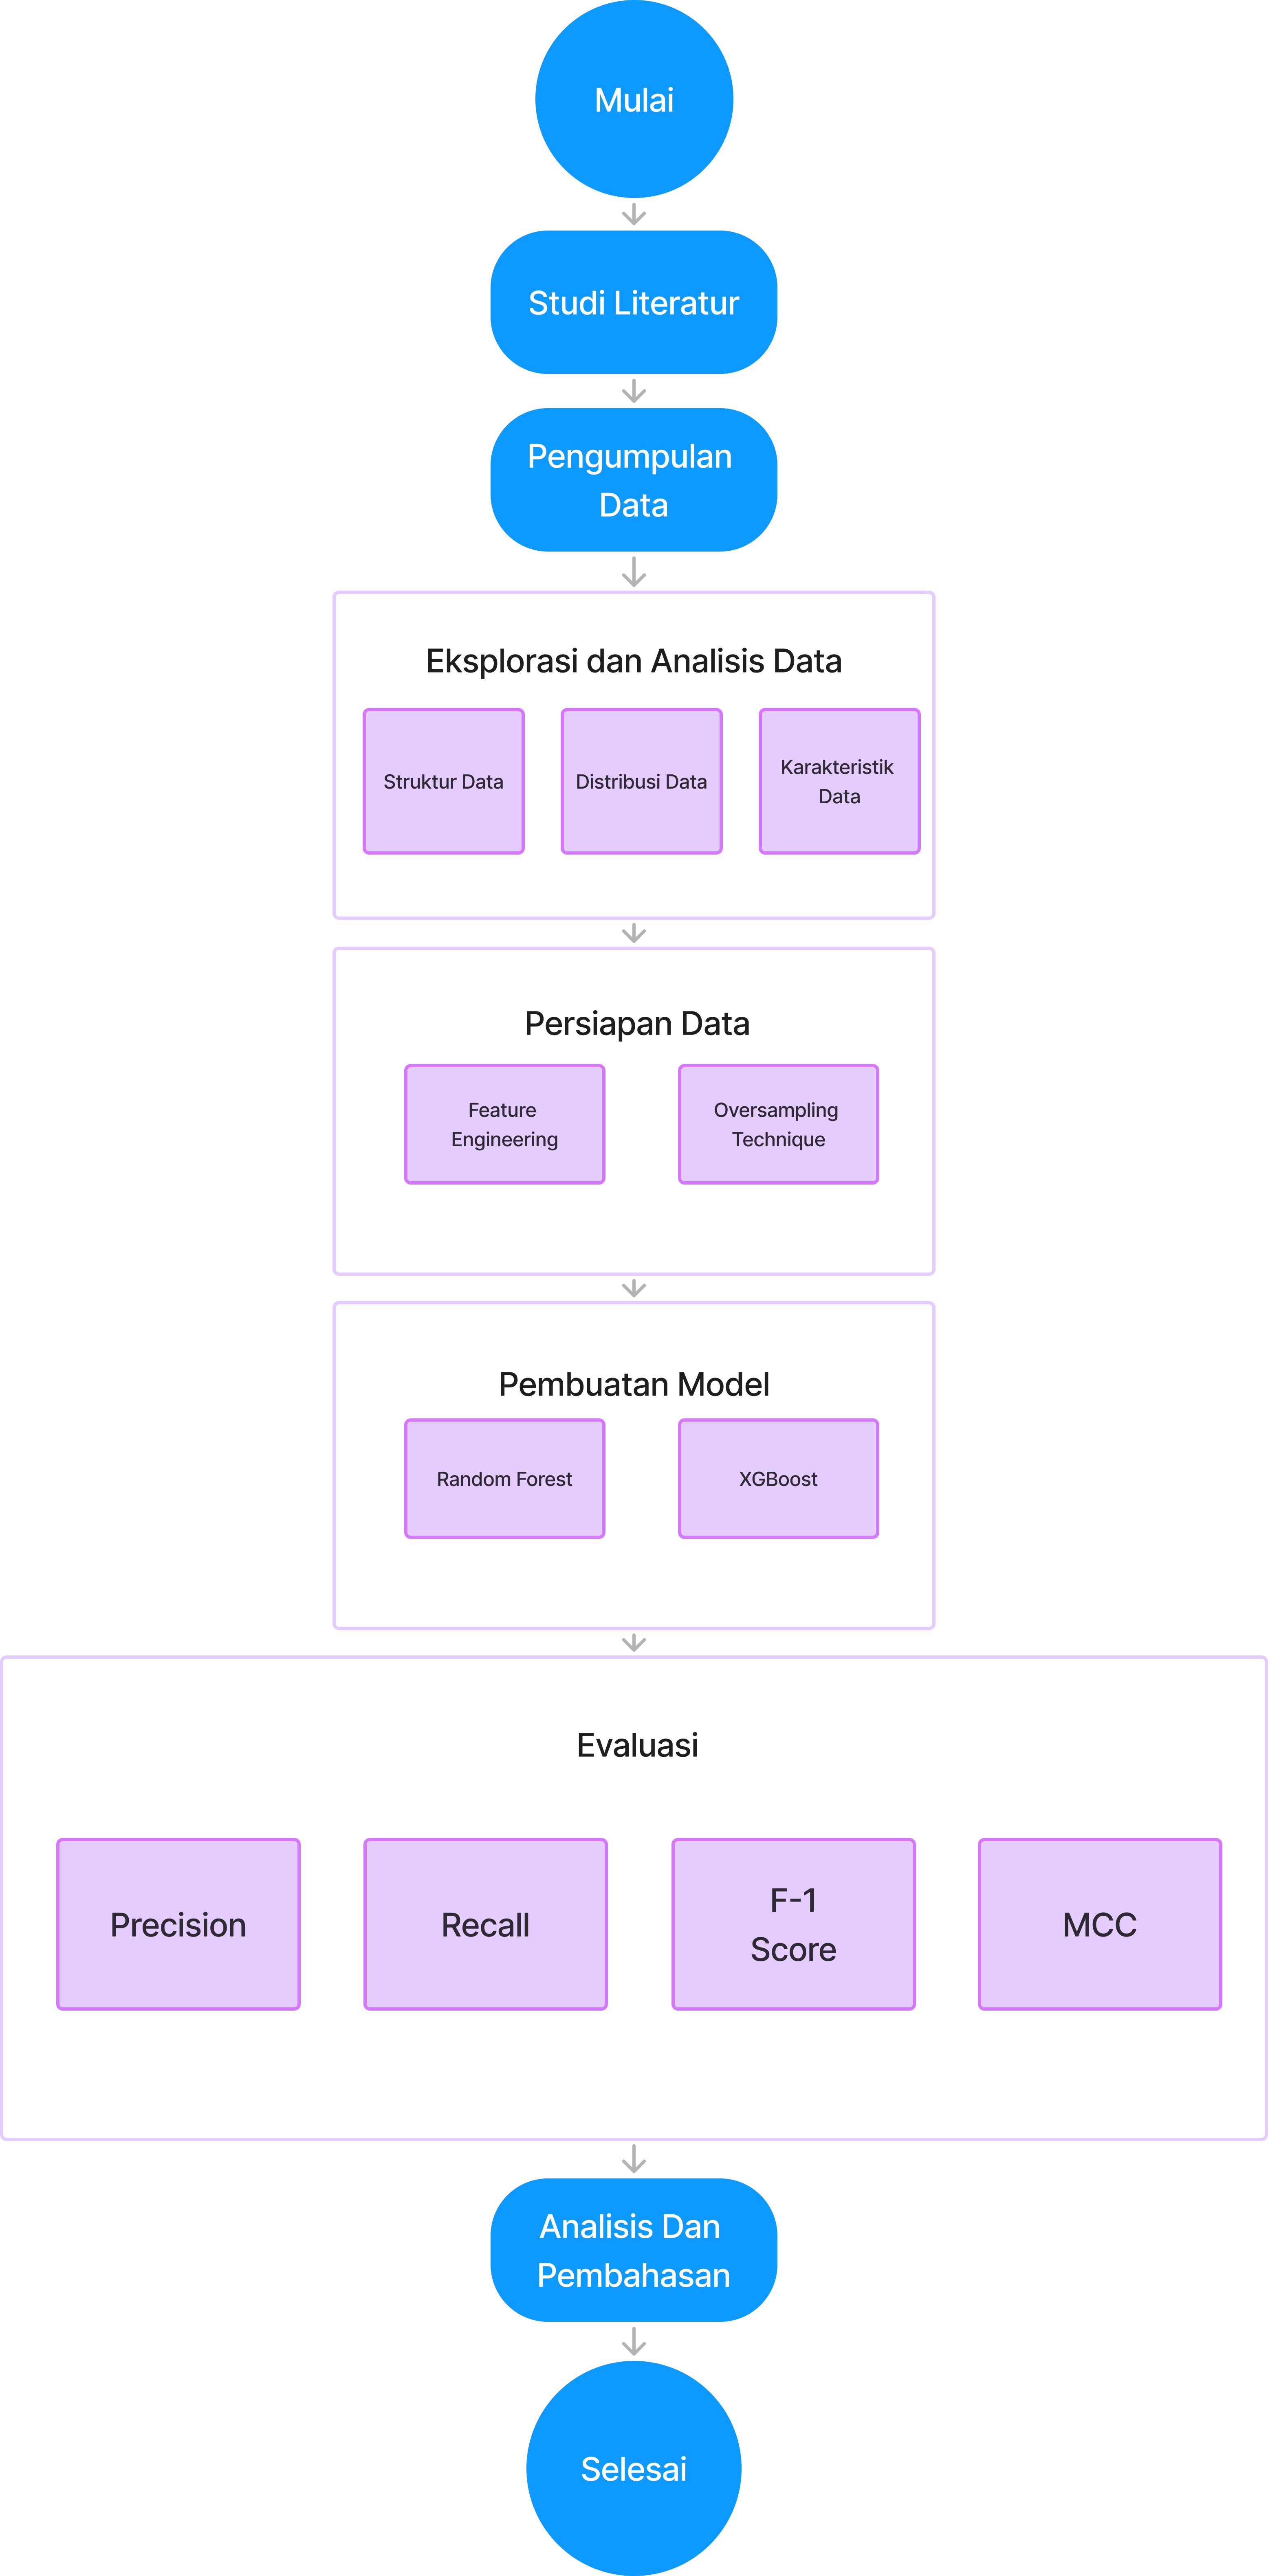
\includegraphics[width=0.5\textwidth]{figure/alur_penelitian.png}
	\caption{Alur Penelitian}
	\label{fig:3.alur penelitian}
\end{figure}

\section{Penjabaran Langkah Penelitian} \label{III.Jabar Alur}
Alur penelitian yang akan dilakukan memiliki beberapa tahapan yang dilakukan secara bertahap dan terdapat sub tahapan pada persiapan data dan juga pembuatan model yang dapat kita lihat pada gambar \ref{fig:3.Skema Pembuatan Model}.
\begin{figure}[H]
	\centering
	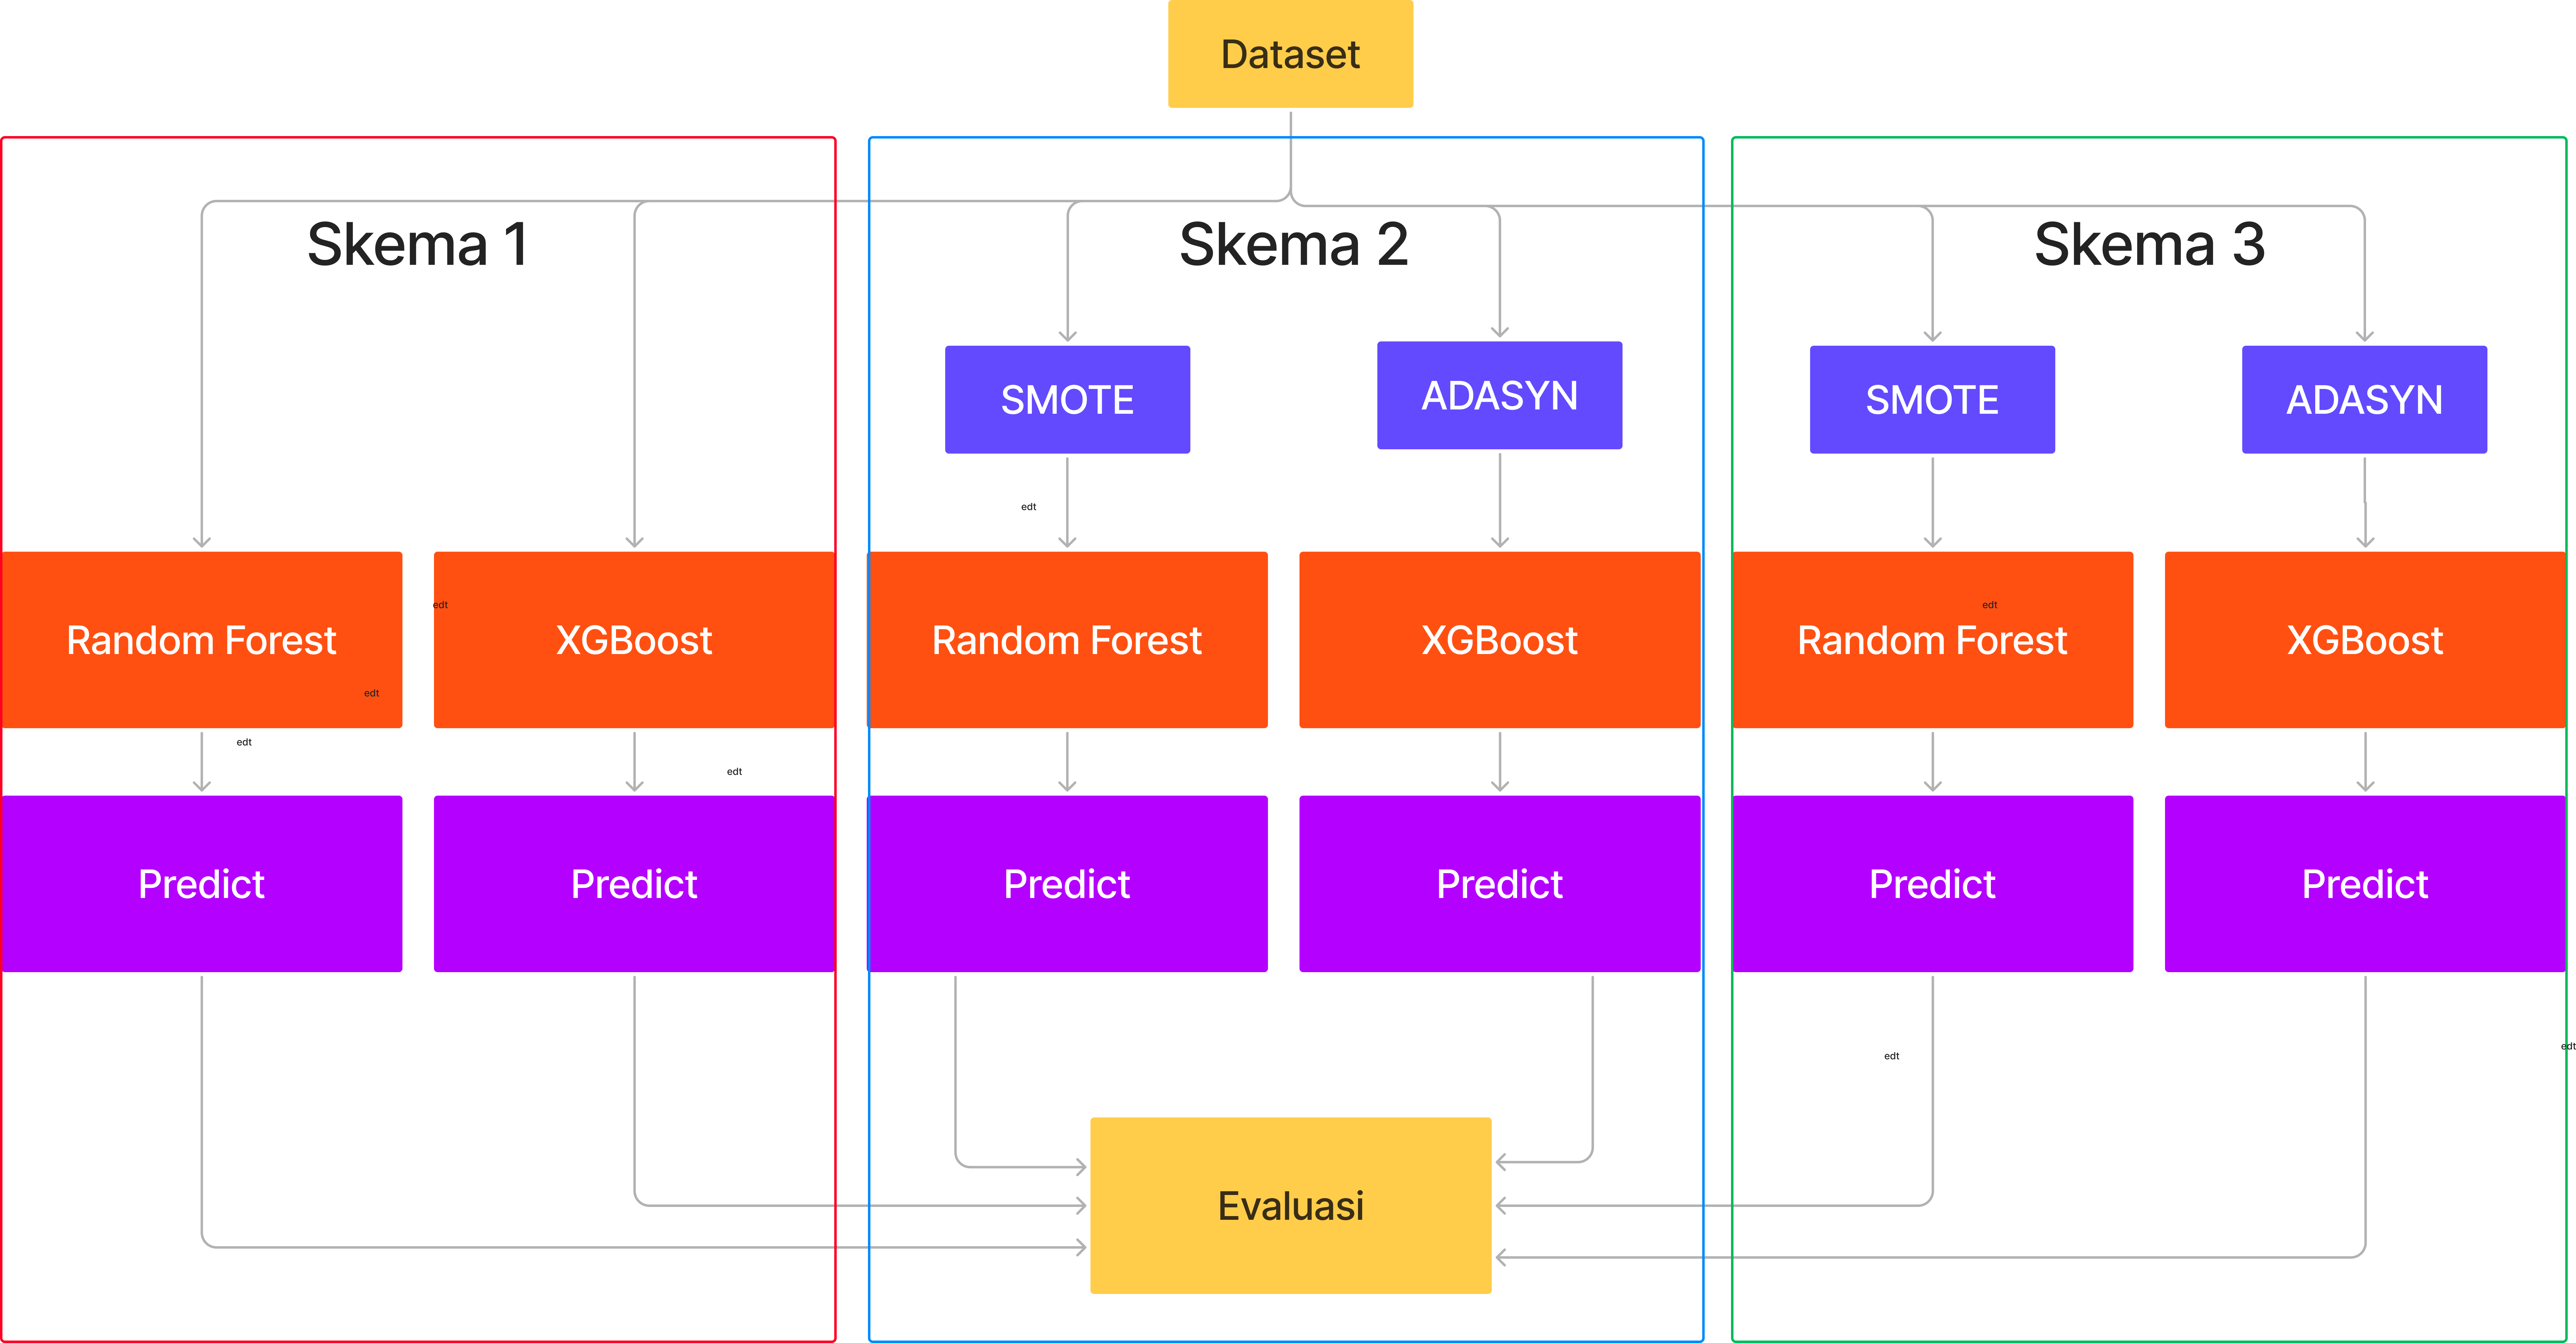
\includegraphics[width=0.7\textwidth]{figure/pembuatanmodel.png}
	\caption{Skema Pembuatan Model}
	\label{fig:3.Skema Pembuatan Model}
\end{figure}

\subsection{Studi Literatur} \label{III.StudiLiteratur}
Proses ini merupakan proses awal yang perlu dilakukan dalam melakukan penilitan guna memahami dan mengetahui teori-teori yang dibutuhkan dalam penelitian. Studi literatur yang dilakukan mencakup algoritma apa yang digunakan dan metode apa yang digunakan dalam membangun model pendeteksi kartu kredit. Hasil dari proses studi literatur yang peneliti lakukan yang berlandasan kepada 6 penelitian yang tinjau pustakanya menunjukan belum adanya analisis yang berfokus kepada teknik oversampling dalam mengatasi transaksi penipuan kartu kredit. Riset-riset sebelumnya banyak berfokus kepada algoritma \textit{machine learning} apa yang digunakan, padahal proses \textit{oversampling} sangat menentukan apakah sebuah algoritma itu bisa berjalan dengan baik atau tidak\cite{ningsih2022analisis}, terkhusus pada kasus deteksi penipuan kartu kredit. \textit{Imbalanced data} pada dataset kartu kredit merupakan hal krusial dalam pembuatan model pendekteksi penipuan kartu kredit dikarenakan dapat membuat model \textit{machine learnng} menjadi bias terhadap kelas minoritas dan salah cara efektif untuk mengatasi masalah hal tersebut ialah dengan menggunakan teknik oversampling\cite{liu2004effect}.
\subsection{Pengumpulan Data} \label{III.pengumpulandata}
Pada proses ini peneliti menggunakan dataset yang dikumpulkan oleh \textit{machine learning group} dari Université Libre de Bruxelles\cite{WinNT,leborgne2022fraud} yang berisi transaksi yang terjadi di eropa. Dataset ini memiliki 492 frauds(penipuan) dari 284.807 transaksi. Dataset ini dipilih oleh peneliti dikarenakan \textit{dataset} tersebut sangat tidak seimbang(\textit{ highly unbalanced}) dengan persentase penipuan sebesar 0.172\% yang dapat dilihat pada gambar \ref{fig:3.Perbandingan Transaksi Normal dan Penipuan} yang membuat dataset tersebut sangat cocok dalam penelitian ini.\\
Dataset tersebut disajikan dalam bentuk file CSV. Dataset tersebut memiliki 30 fitur dan satu label dengan 28 fiturnya sudah dalam bentuk \textit{PCA transformation} guna melindungi privasi data(confidentiality issues) dan 2 fitur lainya tidak dirubah kedalam bentuk PCA adalah \textit{time}, dan \textit{amount} dan untuk label berupa \textit{class}. Fitur 'Time' berisi jumlah detik yang telah berlalu antara setiap transaksi dan transaksi pertama dalam dataset. Fitur 'Amount' merupakan jumlah transaksi. Label 'Class' ini berisi 2 bentuk 1 dan 0 yang mana 1 merupakan \textit{fraud} dan 0 \textit{non-fraud}.
\begin{figure}[H]
	\centering
	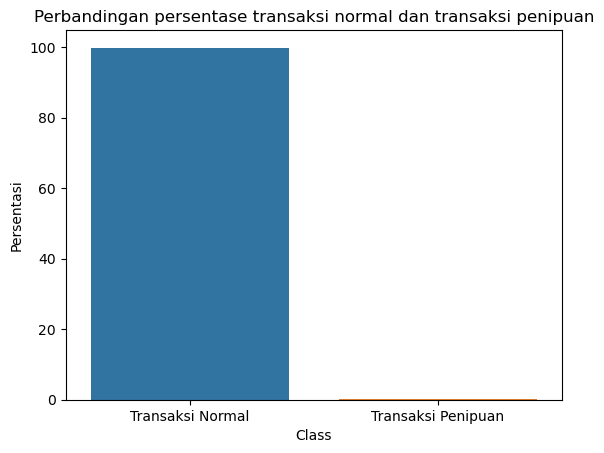
\includegraphics[width=0.5\textwidth]{figure/perbandinganpersentasenormalpenipuan.png}
	\caption{Perbandingan Transaksi Normal dan Penipuan}
	\label{fig:3.Perbandingan Transaksi Normal dan Penipuan}
\end{figure}

\subsection{Eksplorasi dan Analisis Data}
Hasil dari explorasi dan analisis data pada tipe data  dataset \textit{credit card fraud detection} memiliki tipe data \textit{float64} pada hampir semua fiturnya kecuali pada fitur class yang memiliki tipe data \textit{int64} dikarenakan fitur class masih dalam bentuk int64, sebaiknya diubah tipe datanya kedalam bentuk tipe data \textit{category} dikarenakan membuat penggunaan memori menjadi efisien\cite{mckinney2024pandas}. Memori efisien  berpotensi meningkatkan performa dalam \textit{training model}. \\
Peneliti selanjutnya mencoba untuk melakukan analisis dataset pada fitur time dan amount dikarenakan 2 fitur tersebut tidak diubah kedalam bentuk PCA dan peneliti ingin melihat apakah fitur tersebut tetap dipertahankan atau tidak. Pada fitur \textit{time} peneliti akan melakukan observasi distribusi pada transaksi normal dan penipuan berdasarkan waktu dengan menggunakan diagram KDE untuk melihat distribusinya, yang dapat dilihat pada gambar \ref{fig:3.Perbandingan Distribusi Transaksi Normal dan Penipuan Berdasarkan Waktu} yang mana pada figure tersebut bisa kita lihat kalau kedua transaksi normal dan penipuan memiliki distribusi ganda yang memiliki dua puncak yang berarti merupakan \textit{bimodal distribution}\cite{gonick1993cartoon}, hal ini menunjukkan bahwa transaksi dalam dataset terjadi pada dua periode waktu yang berbeda dan setelah itu dapat kita lihat kalau transaksi normal dan penipuan juga merupakan \textit{distribution overlap}\cite{gonick1993cartoon} dikarenakan hal itu kita akan tetap mempertahankan menggunakan \textit{feature} tersebut. 
\begin{figure}[H]
	\centering
	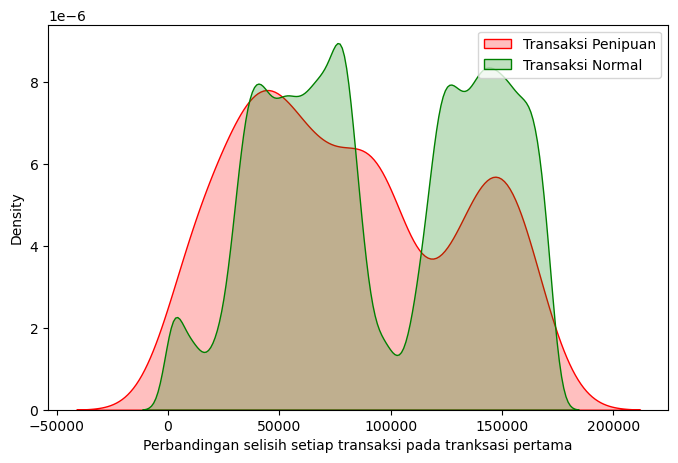
\includegraphics[width=0.5\textwidth]{figure/distribusiwaktunormalpenipuan.png}
	\caption{Perbandingan Distribusi Transaksi Normal dan Penipuan Berdasarkan Waktu}
	\label{fig:3.Perbandingan Distribusi Transaksi Normal dan Penipuan Berdasarkan Waktu}
\end{figure}
Pada fitur \textit{amount} peneliti akan melakukan observasi distribusi pada transaksi normal dan penipuan berdasarkan \textit{amount} yang dilakukan menggunakan diagram KDE sama seperti saat melakukan observasi pada fitur \textit{time}. Berdasarkan hasil observasi distribusi pada gambar \ref{fig:3.Perbandingan Jumlah Transaksi Transaksi Normal dan Penipuan} menunjukan bahwa distribusi dari kedua fitur tersebut merupakan \textit{skewed distribution} yang terpusat pada jumlah transaksi yang rendah(diantara 0 sampai 100) yang dapat kita lihat pada gambar \ref{fig:3.Jumlah Transaksi 0 Sampai 100}. Kedua fitur tersebut merupakan \textit{overlap distribution} namun sedikit perbedaan yang cukup jelas bahwa distribusi transaksi penipuan lebih rendah daripada transaksi normal dan perbedaan selanjutnya pada kedua fitur tersebut ialah transaksi penipuan jarang terjadi pada jumlah transaksi besar(diatas 2500 sampai 25000) yang dapat dilihat pada gambar \ref{fig:3.Jumlah Transaksi 2500 Sampai 25000} dikarenakan banyaknya hubungan yang membedakan transaksi normal dan penipuan, fitur \textit{amount} akan digunakan oleh peneliti.
\begin{figure}[H]
	\centering
	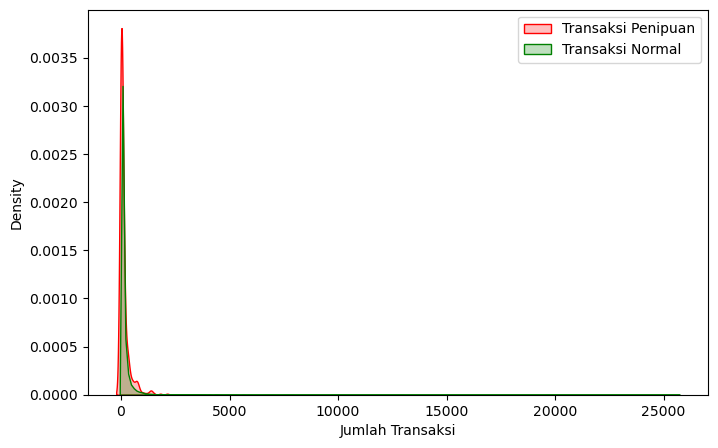
\includegraphics[width=0.5\textwidth]{figure/jumlah transaksi.png}
	\caption{Perbandingan Jumlah Transaksi Transaksi Normal dan Penipuan}
	\label{fig:3.Perbandingan Jumlah Transaksi Transaksi Normal dan Penipuan}
\end{figure}
\begin{figure}[H]
	\centering
	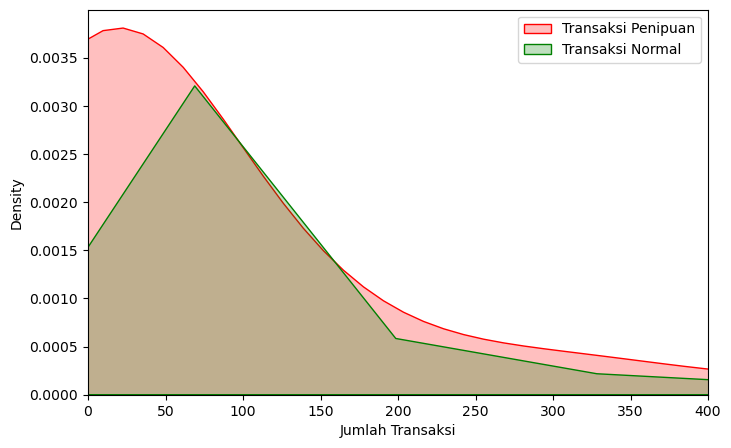
\includegraphics[width=0.5\textwidth]{figure/nolsampaiseratus.png}
	\caption{Jumlah Transaksi 0 Sampai 100}
	\label{fig:3.Jumlah Transaksi 0 Sampai 100}
\end{figure}
\begin{figure}[H]
	\centering
	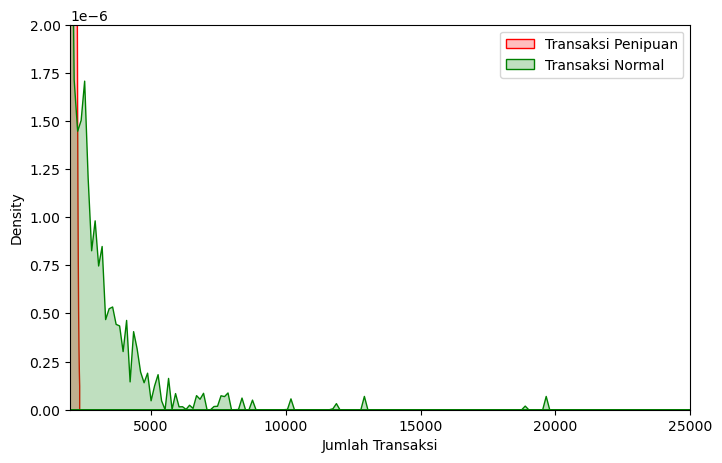
\includegraphics[width=0.5\textwidth]{figure/jumlahtransaksiduaribulimaratus.png}
	\caption{Jumlah Transaksi 2500 Sampai 25000}
	\label{fig:3.Jumlah Transaksi 2500 Sampai 25000}
\end{figure}

\subsection{Persiapan Data}
Proses memuat persiapan data sebelum diinputkan ke dalam \textit{machine learning}. Setelah peneliti melakukan analisis dan eksplorasi data, ada beberapa hal yang perlu dilakukan dalam persiapan data, yang pertama ialah mengecek apakah ada \textit{missing value} didalam dataset, dengan cara mengecek persentase dari setiap feature yang ada pada dataset dengan menggunakan formula berikut:\\

\begin{equation}
       \text{Null\_Percentage}_i = \left( \frac{\sum_{j=1}^{n} \mathbf{1} \{ x_{ij} = \text{null} \}}{n} \right) \times 100
\label{eq:3.missingvalue}
\end{equation}
\myequations{Rumus \textit{missing value}}

Setelah itu peneliti akan melakukan\textit{split} data train dan test dengan metode pengambilan datanya dengan menggunakan \textit{stratified sampling} dengan format 80:20, 80\% data training dan 20\% data test dengan menggunakan modul sklearn model selection dengan melakukan import train\_test\_split. Setelah itu Penelti akan melakukan feature scaling pada feature amount dikarenakan feature amount ukuran nya masih sangat berbeda dibandingkan dengan feature lainya yang sudah dilakukan PCA transformation. Untuk itu, penelti akan melakukan feature scaling dengan menggunakan \textit{Robust Scaling}
dari sklearn. Hasil dari feature scaling pada data training dapat dilihat perubahaannya dari table 3.2 menjadi 3.3.\\
\begin{longtable}{| m{0.6cm} | m{2cm}|}
\caption{5 Data Train Amount Sebelum Scaling} \label{tab:trainingsebelumscaling} \\
\hline
No. & Amount  \\ 
\hline
\endhead
\hline \multicolumn{2}{r}{\textit{Continued}} \\ \hline
\endfoot
\endlastfoot
1 & 7.32  \\ 
\hline
2 & 2.99  \\ 
\hline
3 & 175.10  \\ 
\hline
4 & 6.10  \\ 
\hline
5 & 86.10  \\ 
\hline
\end{longtable}
\begin{longtable}{| m{0.6cm} | m{2cm}|}
\caption{5 Data Train Amount Sesudah Feature Scaling} \label{tab:trainingsesudahscaling} \\
\hline
No. & Amount  \\ 
\hline
\endhead
\hline \multicolumn{2}{r}{\textit{Continued}} \\ \hline
\endfoot
\endlastfoot
1 & 0.000258  \\ 
\hline
2 & 0.000161  \\ 
\hline
3 & 0.006816  \\ 
\hline
4 & 0.000237  \\ 
\hline
5 & 0.003351  \\ 
\hline
\end{longtable}
Selanjutnya peneliti akan melakukan metode \textit{oversampling} yang akan diimplementasikan pada skema 2 dan 3 yang dapat divisualisasikan kedalam plot diagram. namun sebelum itu, agar dapat divisualisasikan kedalam plot diagram yang berupa 2 dimensi data harus diubah dimensinya dikarenakan data yang kita miliki merupakan 30 dimensi, perubahan dimensi tanpa menghilangkan relationship data ialah dengan menggunakan T-SNE dikarenakan T-SNE , hasil dari T-SNE dapat dilihat pada gambar \ref{fig:3.Visualisasi Data TSNE sebelum dan Sesudah SMOTE dan ADASYN}. 
\begin{figure}[H]
	\centering
	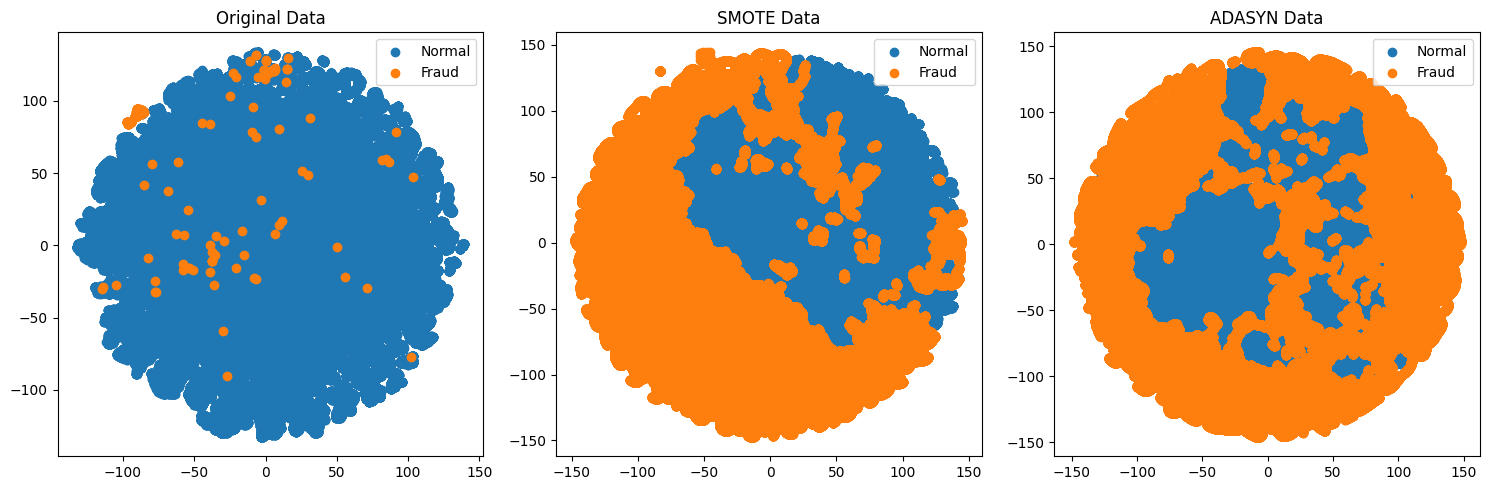
\includegraphics[width=0.7\textwidth]{figure/plot tsne.png}
	\caption{Visualisasi Data TSNE sebelum dan Sesudah SMOTE dan ADASYN}
	\label{fig:3.Visualisasi Data TSNE sebelum dan Sesudah SMOTE dan ADASYN}
\end{figure}

\subsection{Pembuatan Model}
\begin{figure}[H]
	\centering
	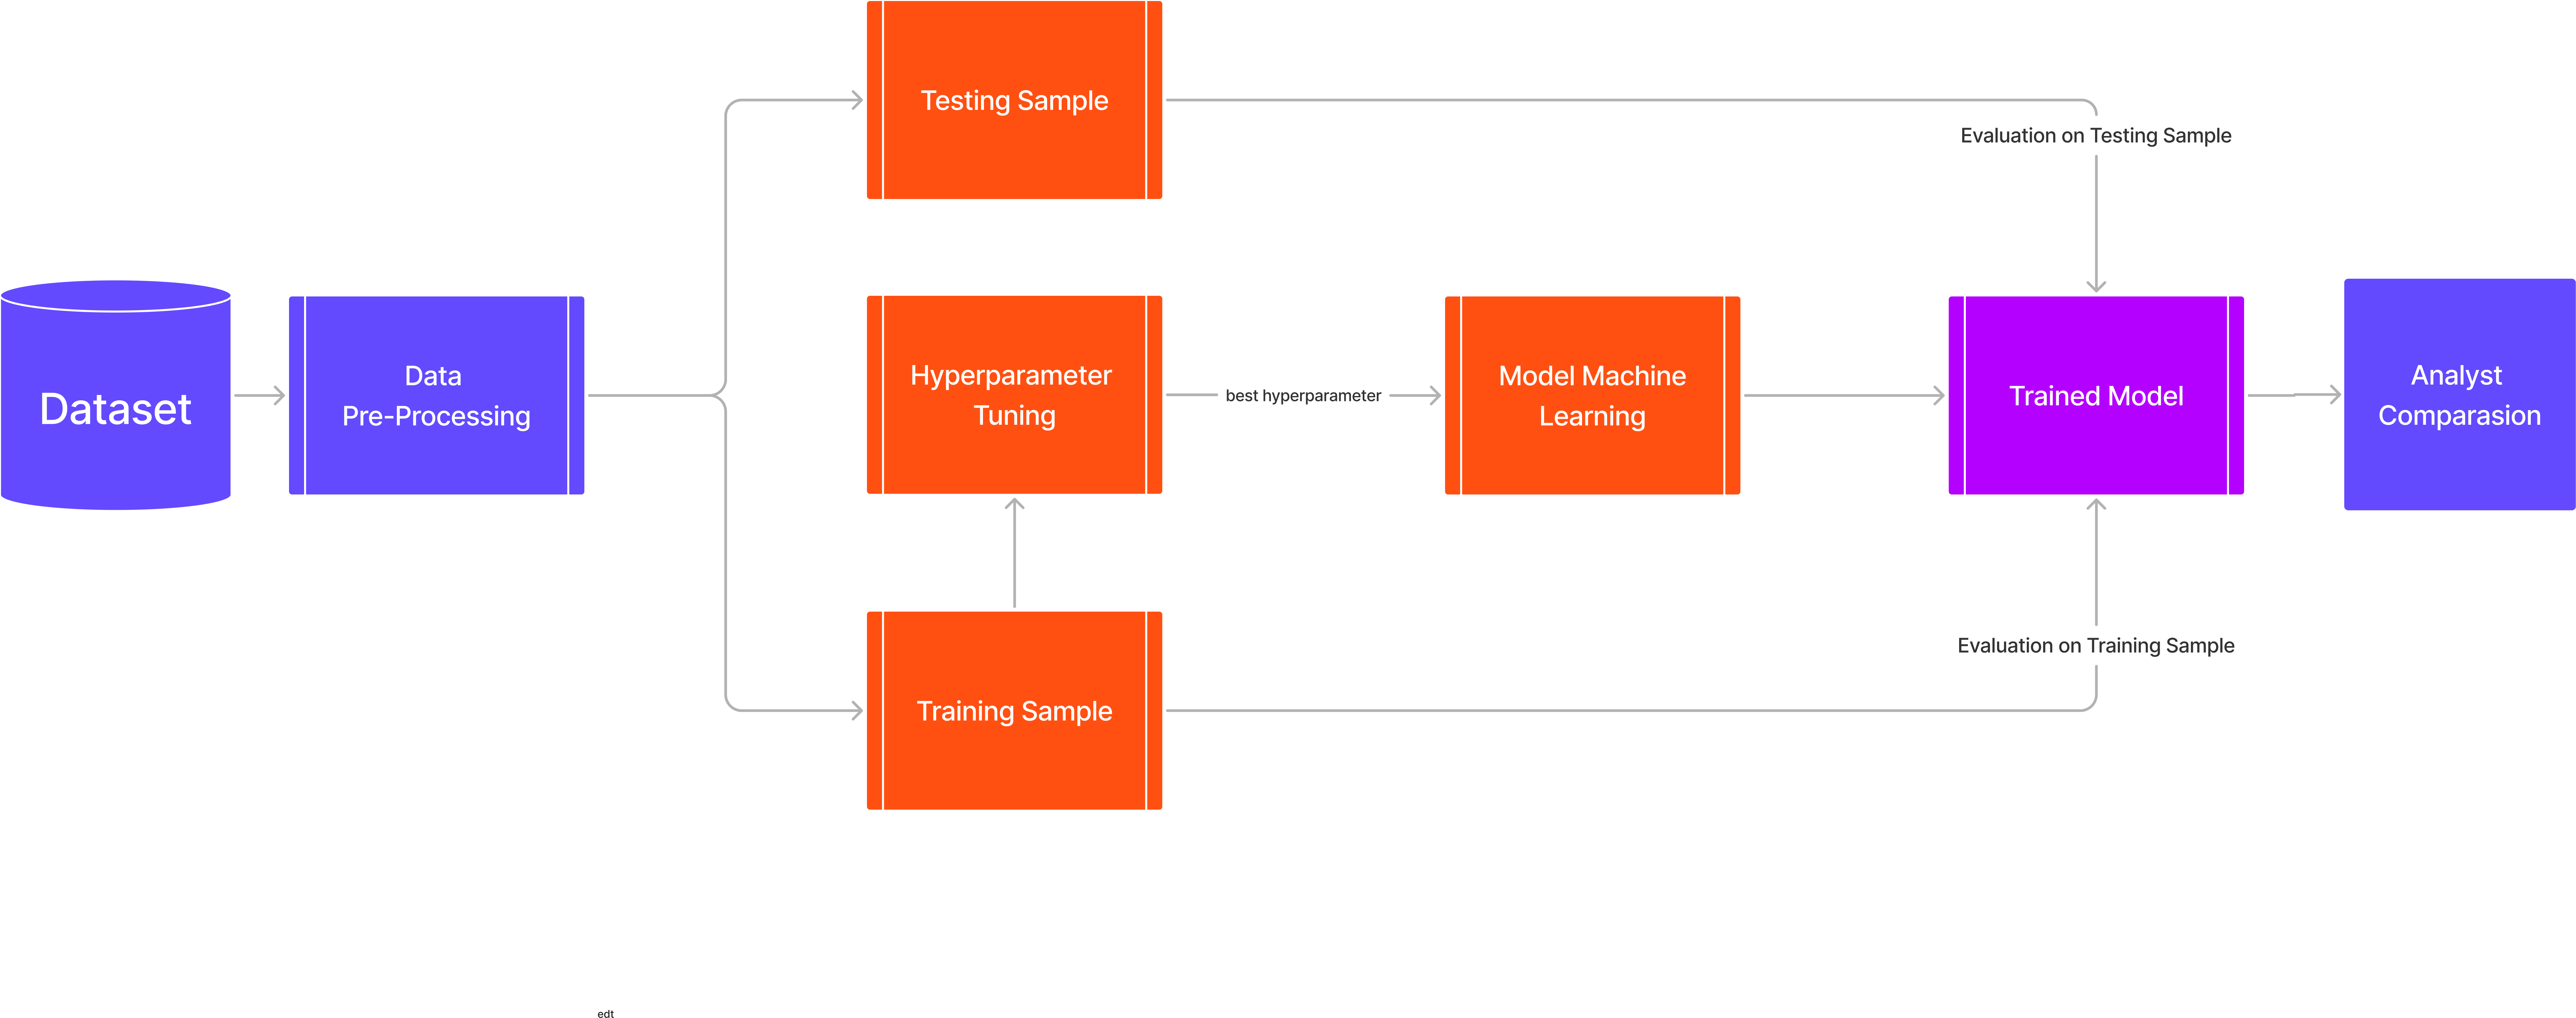
\includegraphics[width=0.7\textwidth]{figure/AlurPembuatanModel.png}
	\caption{Alur Pembuatan Model}
	\label{fig:3.alur pembuatan model}
\end{figure}
Proses ini akan berfokus pada tuning \textit{hyperparameter} model machine learning dengan \textit{cross validation} dengan menggunakan scoring mcc dan melakukan \textit{training model} dengan nilai \textit{hyperparameter} terbaik. Tuning Hyperparameter dilakukan dengan menggunakan \textit{hyperparameter optimization framework} bernama optuna. Pada algoritma \textit{machine learning random forest} \textit{hyperparameter} yang akan dituning berupa\cite{albahli2024efficient}:
\begin{enumerate}[noitemsep]
    \item n\_estimator dengan range nilai dari 200 ke 500.
    \item max\_depth dengan range nilai 5 ke 30.
    \item min\_sample\_split dengan range nilai 5 ke 30.
    \item min\_sample\_leaf dengan range nilai 5 ke 30.
    \item max\_feature dengan pilihan 'auto', 'sqrt', dan 'log2'.
    \item bootstrap dengan pilihan \textit{true} or \textit{false}.
\end{enumerate}
Pada algoritma \textit{machine learning xgboost} \textit{hyperparamter} yang akan dituning dengan menggunakan optuna adalah sebagai berikut\cite{Verma2024ExploringKX}:
\begin{enumerate}[noitemsep]
    \item max\_depth dengan range 3 ke 10.
    \item learning\_rate dengan range 0.01 ke 0.1.
    \item n\_estimator dengan range 200 ke 500.
    \item min\_child\_weight dengan range 3 ke 10.
    \item subsample dengan range 0.6 ke 1.0.
    \item colsample\_bytree dengan range 0.6 ke 1.0.
    \item gamma dengan range 0 ke 1.0.
    \item alpha dengan range 0 ke 5.
\end{enumerate}
Setelah melakukan hyperparameter tuning penelti akan memilih \textit{hyperparameter} terbaik untuk membuat model random forest dan juga xgboost.

\subsection{Evaluasi}
Pengujian dilakukan dengan melihat berdasarkan nilai dari  \textit{precision}, \textit{recall}, \textit{f-1 score}, dan \textit{Matthews’s correlation coefficient} (MCC) pada setiap model yang digunakan dalam penelitian ini seperti \textit{random forest} dan \textit{xgboost}. Evalusi akan dilakukan dengan 4 skenario yaitu dengan membandingkan  hasil skenario tersebut dan setiap skenario akan membuat dua model \textit{random forest} dan \textit{xgboost} dengan metode tertentu.
\begin{enumerate}[noitemsep]
    \item Skenario pertama: Pada skenario pertama peneliti akan melakukan pengecekan performa dari model \textit{random forest} dan \textit{xgboost} tanpa melakukan metode oversampling, yang artinya model dibuat berdasarkan data yang tidak seimbang. Pengecekan perfoma akan dilihat berdasarkan \textit{precision}, \textit{recall},     \textit{f1-score}, dan \textit{Matthews’s correlation coefficient} (MCC) .
    \item Skenario kedua: pada skenario kedua peneliti akan melakukan pengecekan performa dari model \textit{random forest} dan \textit{xgboost} dengan menggunakan metode oversampling SMOTE. Pengecekan perfoma akan dilihat berdasarkan \textit{precision}, \textit{recall},    \textit{f1-score}, dan \textit{Matthews’s correlation coefficient} (MCC).
    \item Skenario ketiga: pada skenario ketiga peneliti akan melakukan pengecekan performa dari model \textit{random forest} dan \textit{xgboost} dengan menggunakan metode oversampling ADASYN. Pengecekan perfoma akan dilihat berdasarkan \textit{precision}, \textit{recall}, \textit{f1-score}, dan \textit{Matthews’s correlation coefficient} (MCC).
    \item Skenario keempat: pada skenario keempat peneliti akan melakukan pengecekan performa secara menyeluruh dengan membandingkan seluruh hasil dari setiap 6 percobaan yang dilakukan dan menentukan hasil percobaan terbaik dengan melihat metriks performa berdasarkan \textit{precision}, \textit{recall}, \textit{f1-score}, dan \textit{Matthews’s correlation coefficient} (MCC).
\end{enumerate}
\subsection{Analisis dan Pembahasan}
Pada tahap in, dilakukan analisis lebih lanjut beserta pembahasan secara detail terhadap pengujian yang telah dilakukan. Setelah melakukan analisis akan dilakukan proses pembahasan dalam bentuk penulisan laporan.


\subsection{Perhitungan SMOTE}
Perhitungan SMOTE dimulai dengan mengetahui data minoritas, sebagai contoh kita memiliki 3 data minortas yaitu:
\begin{enumerate}
	\item Sample A: (2, 3)
	\item Sample B: (4, 7)
	\item Sample C: (3, 4)
\end{enumerate}
Setelah mengetahui data minoritas kita akan mencari \textit{iniitial sample} yang didapatkan dengan melakukan pemilihan acak. Setelah itu, kita akan mencari tetangga terdekat dari \textit{initial sample} ke sampel lainnya dengan menggunakan \textit{Euclidean distance}. Untuk mendapatkan nilai \textit{Euclidean distance} itu dengan menggunakan teorema pythagoras dengan rumus:\\
 \begin{equation}
	 d = \sqrt{(x_2 - x_1)^2 + (y_2 - y_1)^2}
\end{equation}
\label{eq:3.teorema pythagoras}
\\
\myequations{Rumus Teorema Pythagoras}
Kita dapatkan secara acak \textit{intial sample} yaitu sampel A dan selanjutnya kita akan menghitung \textit{Euclidean distance}.
\begin{enumerate}
	\item  Jarak A ke B.\\
		$$
			d_{AB} = \sqrt{(4-2)^2 + (7-3)^2} = \sqrt{2^2 + 4^2} = \sqrt{4 + 16} = \sqrt{20} \approx 4.47
		$$

	\item Jarak A ke C.\\
		$$
			d_{AC} = \sqrt{(3-2)^2 + (4-3)^2} = \sqrt{1^2 + 1^2} = \sqrt{1 + 1} = \sqrt{2} \approx 1.41
		$$
\end{enumerate}
Karena $d_{AC} < d_{AB}$, sampel C merupakan tetangga terdekat dari sampel A. Setelah mengetahui tetangga terdekat, selanjutnya, kita akan membuat data sintetis dengan menggunakan rumus 2.\ref{eq:2.smote}.
\begin{itemize}
	\item Sampel A: (2,3).
	\item Sample C (tetangga terdekat): (3,4).
	\item $\lambda: 0.5$ (dipilih secara acak)
\end{itemize}
Menghitung perbedaan sampel A dan sampel C:
\\
\begin{align*}
    x_{synthetic} &= \text{Sampel A} + \lambda \cdot (\text{Sampel C} - \text{Sampel A})   \\
    x_{synthetic} &= \text{Sampel A} + \lambda \cdot ((3-2), (4-3)) \\
    x_{synthetic} &= \text{Sampel A} + \lambda \cdot (1,1) 
\end{align*}
\\
Mengkalikan dengan lamdha:
\\
\begin{align*}
    x_{synthetic} &= \text{Sampel A} + 0.5 \cdot (1,1) \\ 
    x_{synthetic} &= \text{Sampel A} + (0.5,0.5) 
\end{align*}
\\
Menghasilkan data sintetis:
\\
\begin{align*}
    x_{synthetic} &= (2,3) + (0.5,0.5) \\
    x_{synthetic} &= (2.5, 3.5) 
\end{align*}
\\
data sintetis yang telah berhasil dibuat adalah (2.5, 3.5).
 
\subsection{Perhitungan ADASYN}
Perhitungan ADASYN dimulai dengan mengetahui data mayoritas dan data minoritas. Kita asumsikan kita memliki dataset seperti berikut:
\begin{itemize}
	\item Sampel Minoritas.
		\begin{enumerate}
			\item Sampel A: (2,3).
			\item Sampel B: (3,7).
		\end{enumerate}
	\item Sampel Majoritas.
		\begin{enumerate}
			\item Sampel M1: (2.5, 3.2).
			\item Sampel M2: (2.7, 3.1).
			\item Sample M3: (6,9).
		\end{enumerate}
\end{itemize}
Dan kita akan menginisiasi nilai k(\textit{number of nearest neighbors} = 3 dan total data sintetis yang ingin kita buat adalah 9 $(G = 9)$. Setelah itu kita akan mencari tetangga terdekat dari setiap data minoritas dengan rumus 3.\ref{eq:3.teorema pythagoras}.
Untuk data minortas pada sampel A(2, 3):
\begin{enumerate}
	\item  Jarak A ke M1.\\
		$$
			d_{AM1} = \sqrt{(2.5-2)^2 + (3.2-3)^2} = \sqrt{0.5^2 + 0.2^2} = \sqrt{0.25 + 0.04} = \sqrt{0.29} \approx 0.54
		$$

	\item Jarak A ke M2.\\
		$$
			d_{AM2} = \sqrt{(2.7-2)^2 + (3.1-3)^2} = \sqrt{0.7^2 + 0.1^2} = \sqrt{0.49 + 0.01} = \sqrt{0.50} \approx 0.71 
		$$

	\item Jarak A ke M3.\\
		$$
			d_{AM3} = \sqrt{(6-2)^2 + (9-3)^2} = \sqrt{4^2 + 6^2} = \sqrt{16 + 36} = \sqrt{52} \approx 7.21 
		$$
		
	\item Jarak A ke B.\\
		$$
			d_{AB} = \sqrt{(4-2)^2 + (7-3)^2} = \sqrt{2^2 + 4^2} = \sqrt{4 + 16} = \sqrt{20} \approx 4.47 
		$$
\end{enumerate}
Pada sampel A 3 tetangga terdekat A$(k = 3)$ ialah M1,M2, dan B. yang berarti ratio dari sampel A adalah:

$$
r_A = \frac{Majority}{k} = \frac{2}{3} \approx 0.67
$$
\\
Untuk data minoritas pada sampel B(4, 7):
\begin{enumerate}
	\item  Jarak B ke M1.\\
		$$
			d_{BM1} = \sqrt{(4-2.5)^2 + (7-3.2)^2} = \sqrt{1.5^2 + 3.8^2} = \sqrt{2.25 + 14.44} = \sqrt{16.69} \approx 4.09
		$$

	\item Jarak B ke M2.\\
		$$
		d_{BM2} = \sqrt{(4-2.7)^2 + (7-3)^2} = \sqrt{1.3^2 + 3.9^2} = \sqrt{1.69 + 15.21} = \sqrt{16.9} \approx 4.11 
		$$

	\item Jarak B ke M3.\\
		$$
			d_{BM3} = \sqrt{(4-6)^2 + (7-9)^2} = \sqrt{(-2)^2 + (-2)^2} = \sqrt{4 + 4} = \sqrt{16} \approx 2.83 
		$$
		
	\item Jarak A ke B.\\
		$$
			d_{BA}  \approx 4.47 
		$$
\end{enumerate}
Pada sampel B 3 tetangga terdekat $(k = 3)$ ialah M3,M1, dan M2. yang berarti ratio dari sampel B adalah:

$$
r_B = \frac{Majority}{k} = \frac{3}{3} = 1 
$$
\\
Menentukan alokasi data sintetis:\\
$$
R_total = r_a + r_b = 0.69 + 1 = 1.69
$$
\\
Menghitung \textit{weight} pada setiap minority sampel:

\begin{itemize}
	\item \textit{weight} dari sampel A: \\ 
		$$
			w_A = \frac{r_a}{R_total} = \frac{0.67}{1.67} \approx 0.40
		$$
	\item \textit{weight} dari sampel B:\\
		$$
			w_B = \frac{r_b}{R_total} = \frac{1}{1.67} \approx 0.60
		$$
\end{itemize}

Maka jumlah data sintetis pada masing data minoritas ialah:
\begin{itemize}
	\item Data sintetis pada sampel A:\\
		$$
			G_A = w_A \times G \approx 0.40 \times 9 \approx 3.6 
		$$
	\item Data sintetis pada sample B:\\
		$$
			G_B = w_B \times G \approx 0.60 \times 9 \approx 5.4 
		$$
\end{itemize}
Jumlah dari masing-masing data sintetis ialah 4(dibulatkan) pada sampel A dan 5(dibulatkan) pada sampel B. Setelah mengalokasikan berapa data sintetis yang akan dibuat, dilanjutkan dengan membuat data sintetis pada setiap data minoritas dengan menggunakan rumus 2.\ref{eq:2.smote}. Kita asumsikan bahwa kita memilih secara acak data minoritas dan yang terpilih ialah sampel A dan tetangga terdekat yang terpilih ialah sampel B(karena sampel B merupakan satu-satunya data minoritas lainnya).\\
Menghitung nilai pembeda dari sampel A dan B:\\
\\
\begin{align*}
    x_{synthetic} &= \text{Sampel A} + \lambda \cdot (\text{Sampel B} - \text{Sampel A})   \\
    x_{synthetic} &= \text{Sampel A} + \lambda \cdot ((4-2), (7-3)) \\
    x_{synthetic} &= \text{Sampel A} + \lambda \cdot (2,4) 
\end{align*}
\\
Mengkalikan dengan lamdha $(\lambda = 0.5)$:
\\
\begin{align*}
    x_{synthetic} &= \text{Sampel A} + 0.5 \cdot (2,4) \\ 
    x_{synthetic} &= \text{Sampel A} + (1,2) 
\end{align*}
\\
Menghasilkan data sintetis:
\\
\begin{align*}
    x_{synthetic} &= (2,3) + (1,2) \\
    x_{synthetic} &= (3, 5) 
\end{align*}
\\
data sintetis yang telah berhasil dibuat adalah (3, 5).
 



\subsection{Alat dan Bahan Tugas Akhir}
Adapun alat dan bahan yang digunakan dalam penelitian ini adalah sebagai berikut:
\subsection{Alat}
Berikut adalah alat yang digunakan dalam penelitian ini:
\begin{enumerate}
    \item Spesifikasi Laptop, komputer atau notebook:
    \begin{enumerate}
        \item Minimum spesifikasi komputer, laptop, atau notebook agar dapat melakukan penelitian ini, sebagai berikut:
        \begin{enumerate}
            \item Sistem operasi linux atau  Windows 10 (64-bit), x86-64 based Menggunakan Processor Intel Core i5.
            \item Menggunakan Processor Intel Core i5 atau AMD Ryzen 5.
            \item Kebutuhan RAM paling minimal 8 GB.
            \item Memiliki ruang memori yang bebas setidaknya 10 GB.
        \end{enumerate}
        \item Pada penelitian ini penulis menggunakan laptop dengan spesifikasi sebagai berikut:
        \begin{enumerate}
            \item ubuntu 22.04.4(64-bit),x86\_64 based
            \item AMD Ryzen 5 4600H with Radeon G 
            \item RAM 8.
            \item SSD 512GB
            \item GPU: NVIDIA GeForce GTX 1650 Ti
        \end{enumerate}
    \end{enumerate}
    \item Visual Studio Code
    \item Scikit-Learn
\end{enumerate}
\subsection{Bahan}
Berikut adalah bahan yang digunakan dalam penelitian ini:
\begin{enumerate}
    \item Dataset yang digunakan ialah dataset Credit Card Fraud Detection yang dikumpulkan dan dianalisis oleh \textit{machine learning group} Université Libre de Bruxelles(ULB)
    \item Jurnal penelitian   dari penelitian sebelumnya yang dijadikan dasar teori dan rangkaian konsep serta ide untuk mendukung penelitian.
\end{enumerate}



    % \newpage
\chapter{Hasil dan Pembahasan} \label{Bab IV}

\section{Hasil Penelitian} \label{IV.Hasil}
Berisi hasil penelitian berdasarkan rancangan yang sudah dijelaskan pada Bab \ref{Bab III}, terutama dari Subbab \ref{III.Metode}. Bagi yang membuat alat, jelaskan alat yang jadi dalam bentuk apa. Bagi yang membuat aplikasi, jelaskan aplikasi yang jadi dalam bentuk seperti apa. Jabarkan dalam bentuk pseudocode dan dijelaskan per bagian kodenya. Gunakan gambar dan tabel sebagai alat bantu menjelaskan hasil. \par

\section{Hasil Pengujian} \label{IV.Uji}
Berikan hasil pengujian berdasarkan rancangan \& skenario yang sudah direncanakan sebelumnya pada Subbab \ref{III.Rancang Uji}. \par

\begin{longtable}{|c|c|c|}
	\caption{Contoh Hasil Pengujian}
	\label{table:4.uji}\\
	\hline
	\textbf{Pengujian} & \textbf{Metode A} & \textbf{Metode B} \\
	\hline
	\endhead
	Kecepatan & 10 ms & 12 ms \\ 
	\hline
	Memori & 10 MB & 7 MB \\
	\hline
\end{longtable}

\begin{figure}[H]
	\centering
	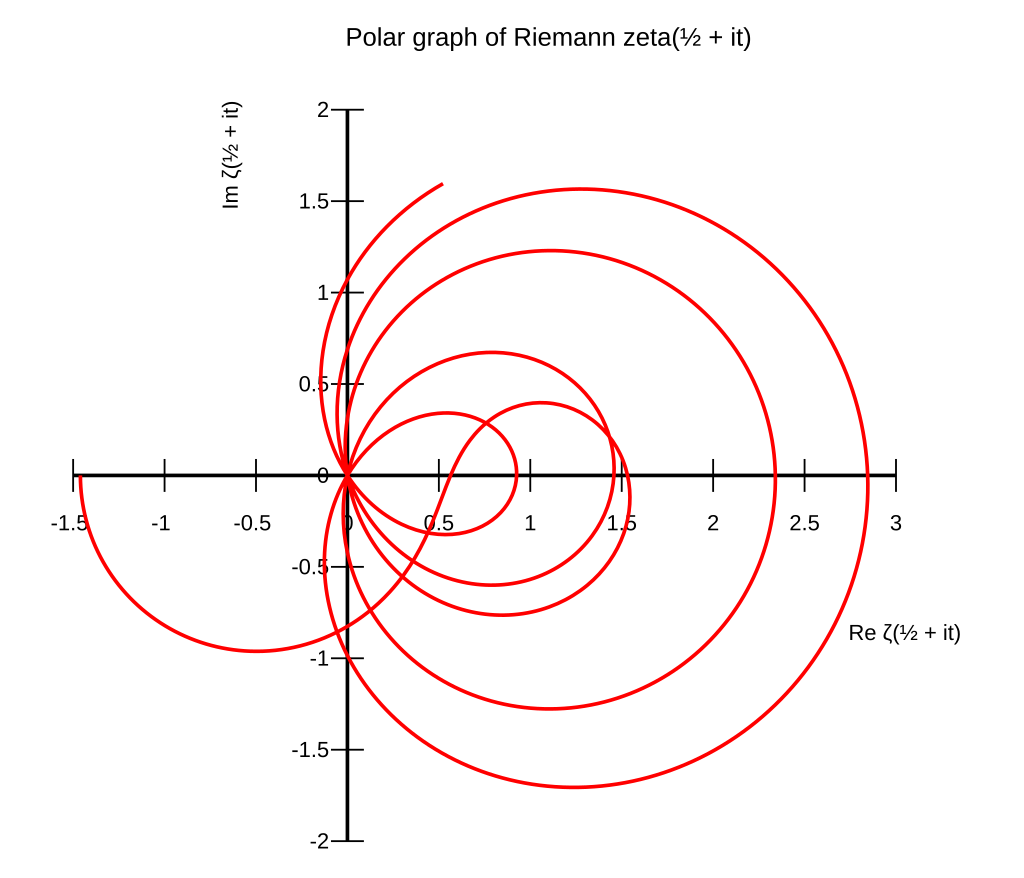
\includegraphics[width=0.5\textwidth]{figure/zeta.png}
	\caption{Contoh Graf Pengujian}
	\label{fig:4.graf}
\end{figure}

\section{Analisis Hasil Penelitian} \label{IV.Analisis}
Berikan analisis hasil penelitian \& pengujian, berupa data yang didapatkan dari penelitian \& pengujian Tugas Akhir yang sudah anda kerjakan. Gunakan gambar dan tabel sebagai alat bantu menjelaskan analisis hasil. Data luaran penelitian yang dapat dianalisis berupa: \par
\begin{enumerate}[noitemsep]
	\item Hasil pengujian
	\item Hasil kuesioner
	\item Aplikasi yang dikembangkan
\end{enumerate}
Analisis dapat membandingkan dengan hasil penelitian sebelumnya yang memiliki kemiripan topik. \par

\section{Pembahasan} \label{IV.Bahas}
Berisi pembahasan terkait hasil yang sudah didapatkan/dipaparkan sebelumnya, berupa penutup yang dapat menjelaskan mengenai kelebihan hasil tugas akhir dan kekurangannya dibandingkan dengan penelitian atau produk lain yang serupa atau mirip. \par
    % \newpage
\chapter{Kesimpulan dan Saran} \label{Bab V}

\section{Kesimpulan} \label{V.Kesimpulan}
Berisi kesimpulan dari hasil dan pembahasan terkait penelitian yang dilakukan, dapat juga berupa temuan yang Anda dapatkan setelah melakukan penelitian atau analisis terhadap tugas akhir Anda. Berhubungan dengan poin pada Subbab \ref{I.Rumusan Masalah} dan \ref{I.Tujuan}. 

\section{Saran} \label{V.Saran}
Berisi saran mengenai aspek Tugas Akhir atau temuan dalam penelitian. Diutamakan saran berdasarkan hasil analisis dari Subbab \ref{IV.Analisis}. Saran dapat dikembangkan dan diperkaya untuk Tugas Akhir selanjutnya. 
    %----------------------------------------------------------------%

    % Daftar Pustaka
    \newpage
    \phantomsection% 
    \addcontentsline{toc}{chapter}{Daftar Pustaka}
    \printbibliography[title={Daftar Pustaka}]

    % Lampiran
    \newpage
    \appendix
    \addcontentsline{toc}{chapter}{Lampiran}
    \chapter*{Lampiran}
    \renewcommand\thesection{\Alph{section}}
    \section{Dataset}
https://www.kaggle.com/datasets/mlg-ulb/creditcardfraud



\end{document}
